% Options for packages loaded elsewhere
\PassOptionsToPackage{unicode}{hyperref}
\PassOptionsToPackage{hyphens}{url}
\PassOptionsToPackage{dvipsnames,svgnames,x11names}{xcolor}
%
\documentclass[
  letterpaper,
  DIV=11,
  numbers=noendperiod]{scrreport}

\usepackage{amsmath,amssymb}
\usepackage{iftex}
\ifPDFTeX
  \usepackage[T1]{fontenc}
  \usepackage[utf8]{inputenc}
  \usepackage{textcomp} % provide euro and other symbols
\else % if luatex or xetex
  \usepackage{unicode-math}
  \defaultfontfeatures{Scale=MatchLowercase}
  \defaultfontfeatures[\rmfamily]{Ligatures=TeX,Scale=1}
\fi
\usepackage{lmodern}
\ifPDFTeX\else  
    % xetex/luatex font selection
\fi
% Use upquote if available, for straight quotes in verbatim environments
\IfFileExists{upquote.sty}{\usepackage{upquote}}{}
\IfFileExists{microtype.sty}{% use microtype if available
  \usepackage[]{microtype}
  \UseMicrotypeSet[protrusion]{basicmath} % disable protrusion for tt fonts
}{}
\makeatletter
\@ifundefined{KOMAClassName}{% if non-KOMA class
  \IfFileExists{parskip.sty}{%
    \usepackage{parskip}
  }{% else
    \setlength{\parindent}{0pt}
    \setlength{\parskip}{6pt plus 2pt minus 1pt}}
}{% if KOMA class
  \KOMAoptions{parskip=half}}
\makeatother
\usepackage{xcolor}
\setlength{\emergencystretch}{3em} % prevent overfull lines
\setcounter{secnumdepth}{5}
% Make \paragraph and \subparagraph free-standing
\ifx\paragraph\undefined\else
  \let\oldparagraph\paragraph
  \renewcommand{\paragraph}[1]{\oldparagraph{#1}\mbox{}}
\fi
\ifx\subparagraph\undefined\else
  \let\oldsubparagraph\subparagraph
  \renewcommand{\subparagraph}[1]{\oldsubparagraph{#1}\mbox{}}
\fi


\providecommand{\tightlist}{%
  \setlength{\itemsep}{0pt}\setlength{\parskip}{0pt}}\usepackage{longtable,booktabs,array}
\usepackage{calc} % for calculating minipage widths
% Correct order of tables after \paragraph or \subparagraph
\usepackage{etoolbox}
\makeatletter
\patchcmd\longtable{\par}{\if@noskipsec\mbox{}\fi\par}{}{}
\makeatother
% Allow footnotes in longtable head/foot
\IfFileExists{footnotehyper.sty}{\usepackage{footnotehyper}}{\usepackage{footnote}}
\makesavenoteenv{longtable}
\usepackage{graphicx}
\makeatletter
\def\maxwidth{\ifdim\Gin@nat@width>\linewidth\linewidth\else\Gin@nat@width\fi}
\def\maxheight{\ifdim\Gin@nat@height>\textheight\textheight\else\Gin@nat@height\fi}
\makeatother
% Scale images if necessary, so that they will not overflow the page
% margins by default, and it is still possible to overwrite the defaults
% using explicit options in \includegraphics[width, height, ...]{}
\setkeys{Gin}{width=\maxwidth,height=\maxheight,keepaspectratio}
% Set default figure placement to htbp
\makeatletter
\def\fps@figure{htbp}
\makeatother
\newlength{\cslhangindent}
\setlength{\cslhangindent}{1.5em}
\newlength{\csllabelwidth}
\setlength{\csllabelwidth}{3em}
\newlength{\cslentryspacingunit} % times entry-spacing
\setlength{\cslentryspacingunit}{\parskip}
\newenvironment{CSLReferences}[2] % #1 hanging-ident, #2 entry spacing
 {% don't indent paragraphs
  \setlength{\parindent}{0pt}
  % turn on hanging indent if param 1 is 1
  \ifodd #1
  \let\oldpar\par
  \def\par{\hangindent=\cslhangindent\oldpar}
  \fi
  % set entry spacing
  \setlength{\parskip}{#2\cslentryspacingunit}
 }%
 {}
\usepackage{calc}
\newcommand{\CSLBlock}[1]{#1\hfill\break}
\newcommand{\CSLLeftMargin}[1]{\parbox[t]{\csllabelwidth}{#1}}
\newcommand{\CSLRightInline}[1]{\parbox[t]{\linewidth - \csllabelwidth}{#1}\break}
\newcommand{\CSLIndent}[1]{\hspace{\cslhangindent}#1}

\usepackage{booktabs}
\usepackage{longtable}
\usepackage{array}
\usepackage{multirow}
\usepackage{wrapfig}
\usepackage{float}
\usepackage{colortbl}
\usepackage{pdflscape}
\usepackage{tabu}
\usepackage{threeparttable}
\usepackage{threeparttablex}
\usepackage[normalem]{ulem}
\usepackage{makecell}
\usepackage{xcolor}
\usepackage{rotating}
\KOMAoption{captions}{tableheading}
\makeatletter
\makeatother
\makeatletter
\@ifpackageloaded{bookmark}{}{\usepackage{bookmark}}
\makeatother
\makeatletter
\@ifpackageloaded{caption}{}{\usepackage{caption}}
\AtBeginDocument{%
\ifdefined\contentsname
  \renewcommand*\contentsname{Table of contents}
\else
  \newcommand\contentsname{Table of contents}
\fi
\ifdefined\listfigurename
  \renewcommand*\listfigurename{List of Figures}
\else
  \newcommand\listfigurename{List of Figures}
\fi
\ifdefined\listtablename
  \renewcommand*\listtablename{List of Tables}
\else
  \newcommand\listtablename{List of Tables}
\fi
\ifdefined\figurename
  \renewcommand*\figurename{Figure}
\else
  \newcommand\figurename{Figure}
\fi
\ifdefined\tablename
  \renewcommand*\tablename{Table}
\else
  \newcommand\tablename{Table}
\fi
}
\@ifpackageloaded{float}{}{\usepackage{float}}
\floatstyle{ruled}
\@ifundefined{c@chapter}{\newfloat{codelisting}{h}{lop}}{\newfloat{codelisting}{h}{lop}[chapter]}
\floatname{codelisting}{Listing}
\newcommand*\listoflistings{\listof{codelisting}{List of Listings}}
\makeatother
\makeatletter
\@ifpackageloaded{caption}{}{\usepackage{caption}}
\@ifpackageloaded{subcaption}{}{\usepackage{subcaption}}
\makeatother
\makeatletter
\@ifpackageloaded{tcolorbox}{}{\usepackage[skins,breakable]{tcolorbox}}
\makeatother
\makeatletter
\@ifundefined{shadecolor}{\definecolor{shadecolor}{rgb}{.97, .97, .97}}
\makeatother
\makeatletter
\makeatother
\makeatletter
\makeatother
\ifLuaTeX
  \usepackage{selnolig}  % disable illegal ligatures
\fi
\IfFileExists{bookmark.sty}{\usepackage{bookmark}}{\usepackage{hyperref}}
\IfFileExists{xurl.sty}{\usepackage{xurl}}{} % add URL line breaks if available
\urlstyle{same} % disable monospaced font for URLs
\hypersetup{
  pdftitle={Equitable Access to Nutrition in Utah},
  pdfauthor={Gregory S. Macfarlane; Emma Stucki; Myrranda Salmon; Alisha H. Redelfs; Lori Spruance},
  colorlinks=true,
  linkcolor={blue},
  filecolor={Maroon},
  citecolor={Blue},
  urlcolor={Blue},
  pdfcreator={LaTeX via pandoc}}

\title{Equitable Access to Nutrition in Utah}
\author{Gregory S. Macfarlane \and Emma Stucki \and Myrranda
Salmon \and Alisha H. Redelfs \and Lori Spruance}
\date{2023-09-01}

\begin{document}
\maketitle
\begin{abstract}
Convenient access to high-quality nutrition is a critical element of
public health as well as an important interface between communities and
the transportation system. In this research, we seek to construct a
detailed picture of the nutrition environment in three communities in
Utah, alongside the community members' ability to access that
environment through multiple transportation modes. In doing so we
construct a utility-based accessiblity model enabled by modern mobility
device data. This model reveals the tradeoffs between the quality and
price of goods on one hand and the distance traveled to reach them on
the other. We then apply this model to a series of potential
access-improving policies: building a new store, improving an existing
store, and improving the non-automobile transport network between
residents and existing stores. The results show that new or improved
store locations bring substantially higher benefits than improvements to
the transportation system, at likely lower costs. The report recommends
that UDOT work to increase the availability of community-sized grocery
stores in low-access areas, and consider activity-based methods of
measuring resource access.
\end{abstract}
\ifdefined\Shaded\renewenvironment{Shaded}{\begin{tcolorbox}[enhanced, frame hidden, breakable, sharp corners, interior hidden, borderline west={3pt}{0pt}{shadecolor}, boxrule=0pt]}{\end{tcolorbox}}\fi

\renewcommand*\contentsname{Table of contents}
{
\hypersetup{linkcolor=}
\setcounter{tocdepth}{2}
\tableofcontents
}
\bookmarksetup{startatroot}

\hypertarget{introduction}{%
\chapter{Introduction}\label{introduction}}

The Utah Department of Transportation (UDOT) recently adopted a new
mission to ``Enhance the Quality of Life through Transportation,''
alongside a four-part framework: Better Mobility, Good Health, Connected
Communities, and Strong Economies (UDOT, 2023a). A critical role of the
transportation system in accomplishing all elements of UDOT's mission is
ensuring that all Utah households have adequate access to quality
nutrition and other community resources. Access to quality nutrition is
shown to have a correlation with mental and physical well being (Francis
et al., 2012), and there are many communities that do not have good
accessibility to quality nutrition, with the main options being either
more expensive for quality goods, or no quality goods available.

``Accessibility'' is an abstract concept without a specific quantitative
definition (Handy and Niemeier, 1997). However, using accessibility as a
policy measure requires comparative quantification, and transportation
and public health researchers have constructed several quantitative
measures. Some commonly used measures include:

\begin{itemize}
\tightlist
\item
  Nearest destination: How close is the nearest grocery store?
\item
  Opportunities within a travel time: How many grocery stores can be
  reached within 30 minutes?
\end{itemize}

These types of measures require the researcher to make a series of
assumptions and assertions: why is 30 minutes chosen instead of 40? Is
that time by transit or highway or walking? Should these definitions
change for individuals in different socioeconomic groups? And do people
always go to the closest grocery store to begin with? How much further
are people willing to travel to go to a store that is cheaper or that
has a wider variety of goods? A measure that combines all of these
different considerations is desirable.

\hypertarget{objectives}{%
\section{Objectives}\label{objectives}}

The objective of this project is to develop an understanding of what
variables and attributes are desirable in grocery stores for populations
in different areas of Utah, in order to help identify where to make
improvements to increase equitable access to nutrition in Utah. The
proposed logit model methodology is developed from a connection between
three extensive data sources:

\begin{itemize}
\tightlist
\item
  A detailed survey of the nutrition market in three Utah communities
\item
  Location-based services data derived from mobile phone records
  revealing which grocery stores are frequented by residents of
  different neighborhoods
\item
  Multi-modal network data providing detailed mobility data by car,
  walking, and public transit.
\end{itemize}

These data will be combined in order to develop accurate logit models
that demonstrate the variables that are significant to grocery store
choice in Utah. These models could then be used to find accessibility to
stores and impact transportation policy to improve quality of life for
all communities in Utah.

\hypertarget{outline}{%
\section{Outline}\label{outline}}

This document is organized in a typical manner.
Chapter~\ref{sec-literature} presents a review of transportation
organizations' efforts to improve general health outcomes in their
communities, followed by a specific review of research exploring the
relationship between nutrition access and health. The methodology for
data collection and modeling is described in Chapter~\ref{sec-methods}
and a description of the nutrition environment and choice models
estimates follows in Chapter~\ref{sec-results}.
Chapter~\ref{sec-scenarios} presents a series of scenarios to which we
apply the models estimated in Chapter~\ref{sec-results}, illustrating
the interrelated elements of nutrition quality and transportation
infrastructure in developing more complete access to nutrition. The
document concludes in Chapter~\ref{sec-conclude} with a list of
limitations and a pair of recommendations to UDOT.

\bookmarksetup{startatroot}

\hypertarget{sec-literature}{%
\chapter{Literature Review}\label{sec-literature}}

This chapter presents an overview of existing transportation energy
policies related to health broadly, followed by a review of the
literature on access to nutrition specifically.

\hypertarget{existing-transportation-and-health-policies}{%
\section{Existing Transportation and Health
Policies}\label{existing-transportation-and-health-policies}}

Transportation policy impacts the way our transportation systems
function in cities, and along with that, impacts the way that we live
our lives as well. For example, transportation policy that demands a
certain level of safety on roadways creates a better, safer, travel
network for those using the roads. Also, policy that puts the pedestrian
first helps improve the quality and quantity of sidewalks and bike ways
in cities, improving active transportation. There are many different
types of policies that can be established, whether they be required by
federal law, or established through the individual decisions of local or
state governments. Because these policies make such a big impact on the
way we live it is important to discover what types of policies exist
currently, where there are areas that are missing in policy and
practice, and discover how this research can help to bridge the gap
between identified need and practical application.

How UDOT and other departments of transportation (DOTs) approach their
responsibility to improve quality of life beyond providing mobility is a
relatively recent concern. In this section, we discuss how DOTs have
begun incorporating public health concerns into their policy making and
project prioritization processes.

Transportation impacts public health across several different sectors
identified in the literature, which have been grouped together into four
general topics: Traffic Safety, Pollution, Active Transportation, and
Access to Community Resources. These four topics mirror the focus points
of the UDOT mission, with Traffic Safety and Pollution corresponding to
Good Health, Active Transportation corresponding to Better Mobility, and
Access to Community Resources corresponding to Connected Communities and
Strong Economies.

\hypertarget{traffic-safety}{%
\subsection{Traffic Safety}\label{traffic-safety}}

Arguably the area where most attention has been given in terms of a
public health perspective informing transportation decision making
concerns vehicle and roadway safety. This attention is deserved, as
transportation safety is a major public health concern. In 2021 there
were 329 total fatalities and 1734 serious injuries resulting from car
crashes in Utah, the highest mark in a decade (UDOT, 2023b); though
crashes in 2022 were marginally lower, they still greatly exceeded the
annual rates prior to 2020.

Efforts to improve traffic safety in policy take various forms. One of
the strategies to improve safety focuses on educating the public to
minimize reckless and distracted driving. Research clearly shows the
danger of both reckless and distracted driving and we have recently seen
a national focus on eliminating distracted driving National Highway
Traffic Safety Administration (2022). In response, Utah has implemented
the Zero Fatalities program, focusing on decreasing the number of
roadway fatalities to zero by educating the public on deadly driving
behaviors, including distracted driving, aggressive driving, drowsy
driving, impaired driving, and not wearing seat belts (Zero Fatalities,
2022). Zero Fatalities has different age-specific educational materials
for students and teachers. These age groups include pre-drivers, newly
licensed teenagers, experienced drivers, and even driving instructors.
But, educating the public does not solve all safety concerns; if the
roadways themselves are not safe for the drivers, there needs to be a
change to those roadways as well.

Efforts to change the roadways have focused on improving facilities
design to enhance safety for cars as well as for bikes and pedestrians
(Charreire et al., 2021; Jarry and Apparicio, 2021; Monfort et al.,
2021). In 2012 the Federal Highway Administration established a federal
aid program titled the Safe System Approach that focuses on different
programs including the Strategic Highway Safety Plan (SHSP), Highway
Safety Improvement Program (HSIP), Railroad-Highway Crossings Program
(RHCP), and High Risk Rural Roads (HRRR) (Finkel et al., 2020). Of these
four programs included in the safe system approach, the HSIP is the only
one mandated and implemented in every state, including Utah. The HSIP
gives federal funding for projects, plans, activities, and reports that
improve safety of highways.

Vision Zero (Vision Zero Network, 2022) is a safety program funded by a
non-profit organization that has been implemented in many communities
and combines improving facilities and educating the public. Vision Zero
is a tool to help communities create action plans and strategies. In
order to be involved in Vision Zero the following must be true:

\begin{itemize}
\tightlist
\item
  the community must have a clear goal and plan with a process in place
  to accomplish the goals (including a target date for when the
  community will reach zero fatalities)
\item
  the community leader must declare that they are joining the Vision
  Zero community to strive for zero fatalities on the roadway.
\end{itemize}

This program is a multinational road traffic safety program with the
potential to greatly improve traffic safety in communities where it is
implemented. The Vision Zero focus is to eliminate traffic fatalities
and severe injuries with a clear strategy or plan. A map showing the
communities involved is in Figure~\ref{fig-visionzero}. Vision Zero has
not been implemented in any communities in Utah. Two major differences
between Vison Zero and Utah's Zero Fatalities program are that Zero
Fatalities does not yet have a specific target date of when the state
will reach zero fatalities, and Vision Zero typically includes many
stakeholders such as transportation professionals, policy makers, public
health officials, police, and community members.

\begin{figure}[t]

{\centering 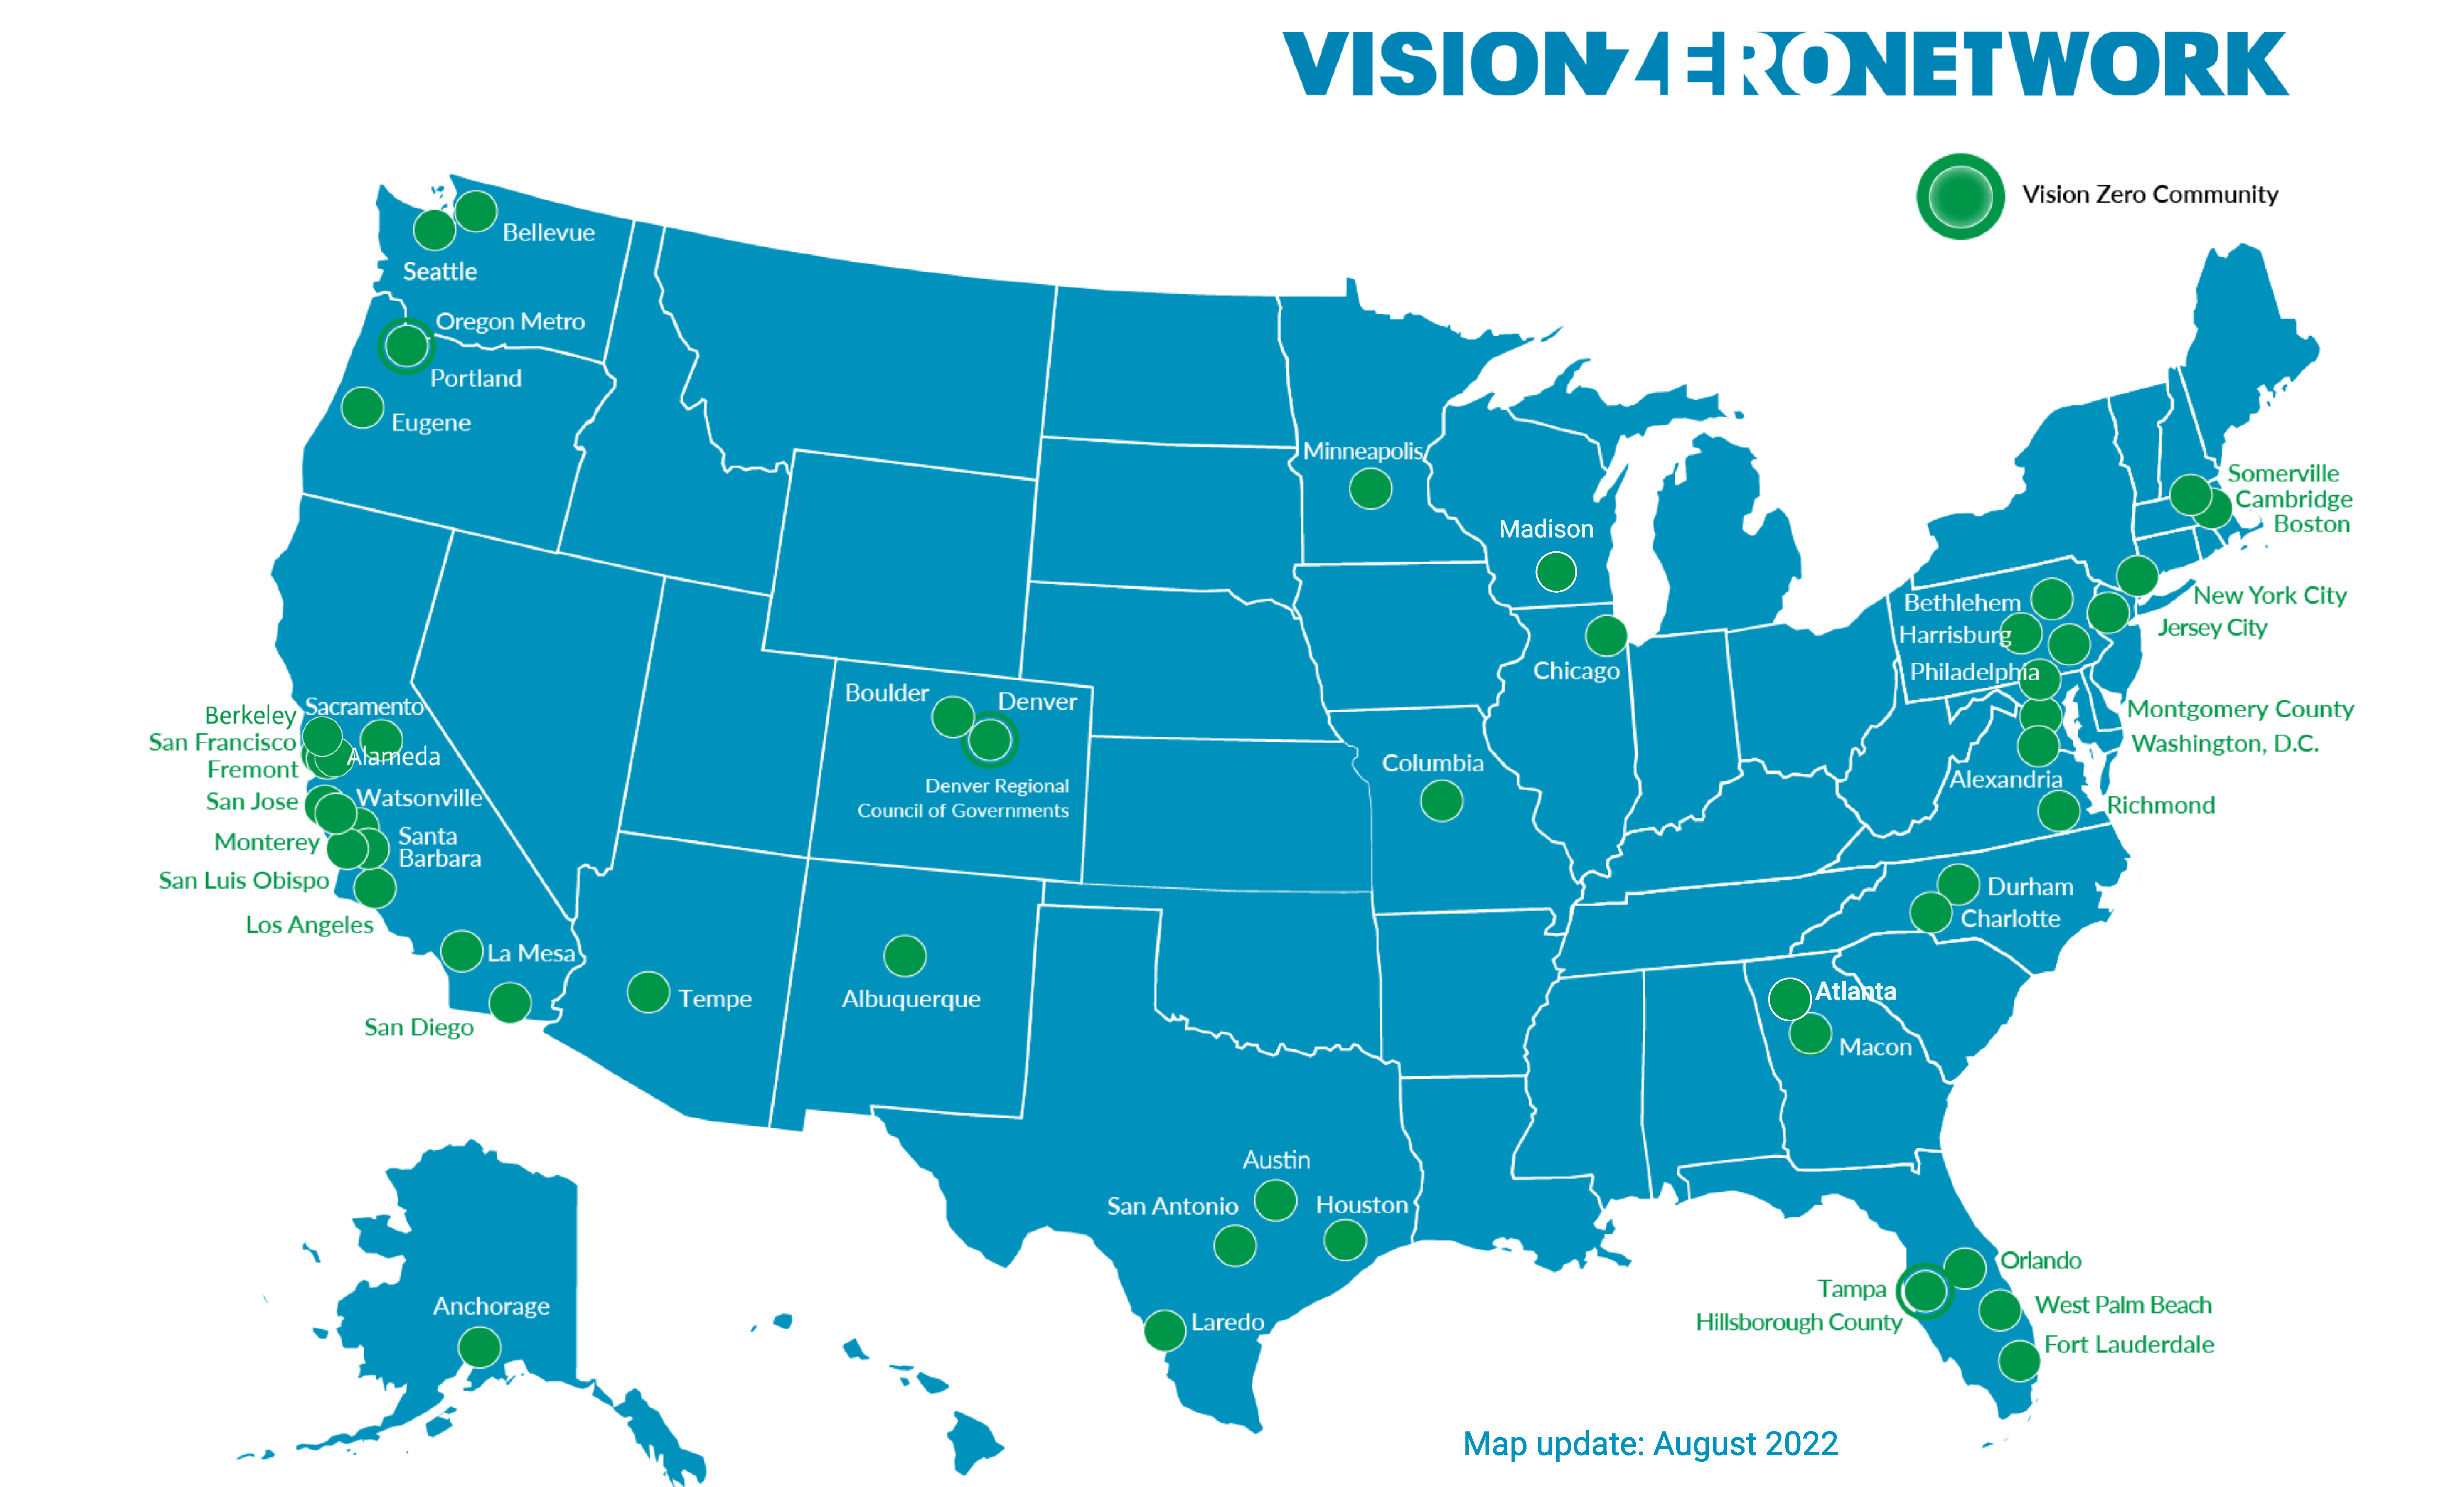
\includegraphics[width=6in,height=\textheight]{images/Vision_Zero_Network_Community_Map_August_2022.png}

}

\caption{\label{fig-visionzero}Vision Zero communities in the United
States.}

\end{figure}

\hypertarget{pollution-and-environmental-justice}{%
\subsection{Pollution and Environmental
Justice}\label{pollution-and-environmental-justice}}

Another place where transportation and public health intersect is
pollution and related environmental justice issues. A large percentage
of airborne pollution comes from vehicle emissions including over 55\%
of nitrogen oxides (NOx), less than 10\% of volatile organic compounds
(VOC), and less than 10\% of particulate matter (PM). Vehicle emissions
are of the largest contributors to PM2.5 levels around the globe.
Studies have shown the impact of fine particulate matter (PM2.5) and
ozone levels on health and have found about 36,000 deaths a year
attributed to these levels Fann et al. (2013). In addition, PM2.5 has
been linked to various health defects such as respiratory and cardiac
symptoms, and exacerbate many other health conditions (Schraufnagel et
al., 2019).

Vehicle pollution has been addressed differently across states.
California has a Zero-Emission Vehicles (ZEVs) strategy to increase the
access of electric vehicle chargers along the roadway networks, support
local transit transitions to zero-emission technology, and support the
development of zero-emission freight technology. Delaware established a
Strategic Implementation Plan for Climate Change, Sustainability and
Resilience for Transportation, and Massachusetts has begun a new Low
Emission Vehicle Program requiring most new vehicles to be equipped with
advanced emission control systems. Utah has implemented a Noise
Abatement Policy to decrease noise pollution which complies with federal
regulation according to NEPA to be environmentally responsible.

On a national level, however, the Clean Air Act directs the
Environmental Protection Agency to set certain quality standards for
pollutants in the air (Environmental Protection Agency, 2023). States
are required to meet these standards or develop a plan to improve
pollution levels. The map in Figure~\ref{fig-nonattainment} shows
counties in each state that do not meet the standard for the identified
air pollutants. As can be seen, there are several counties in Utah that
do not meet the federal air quality standards for certain particulates,
so there are opportunities for improvement.

\begin{figure}[t]

{\centering 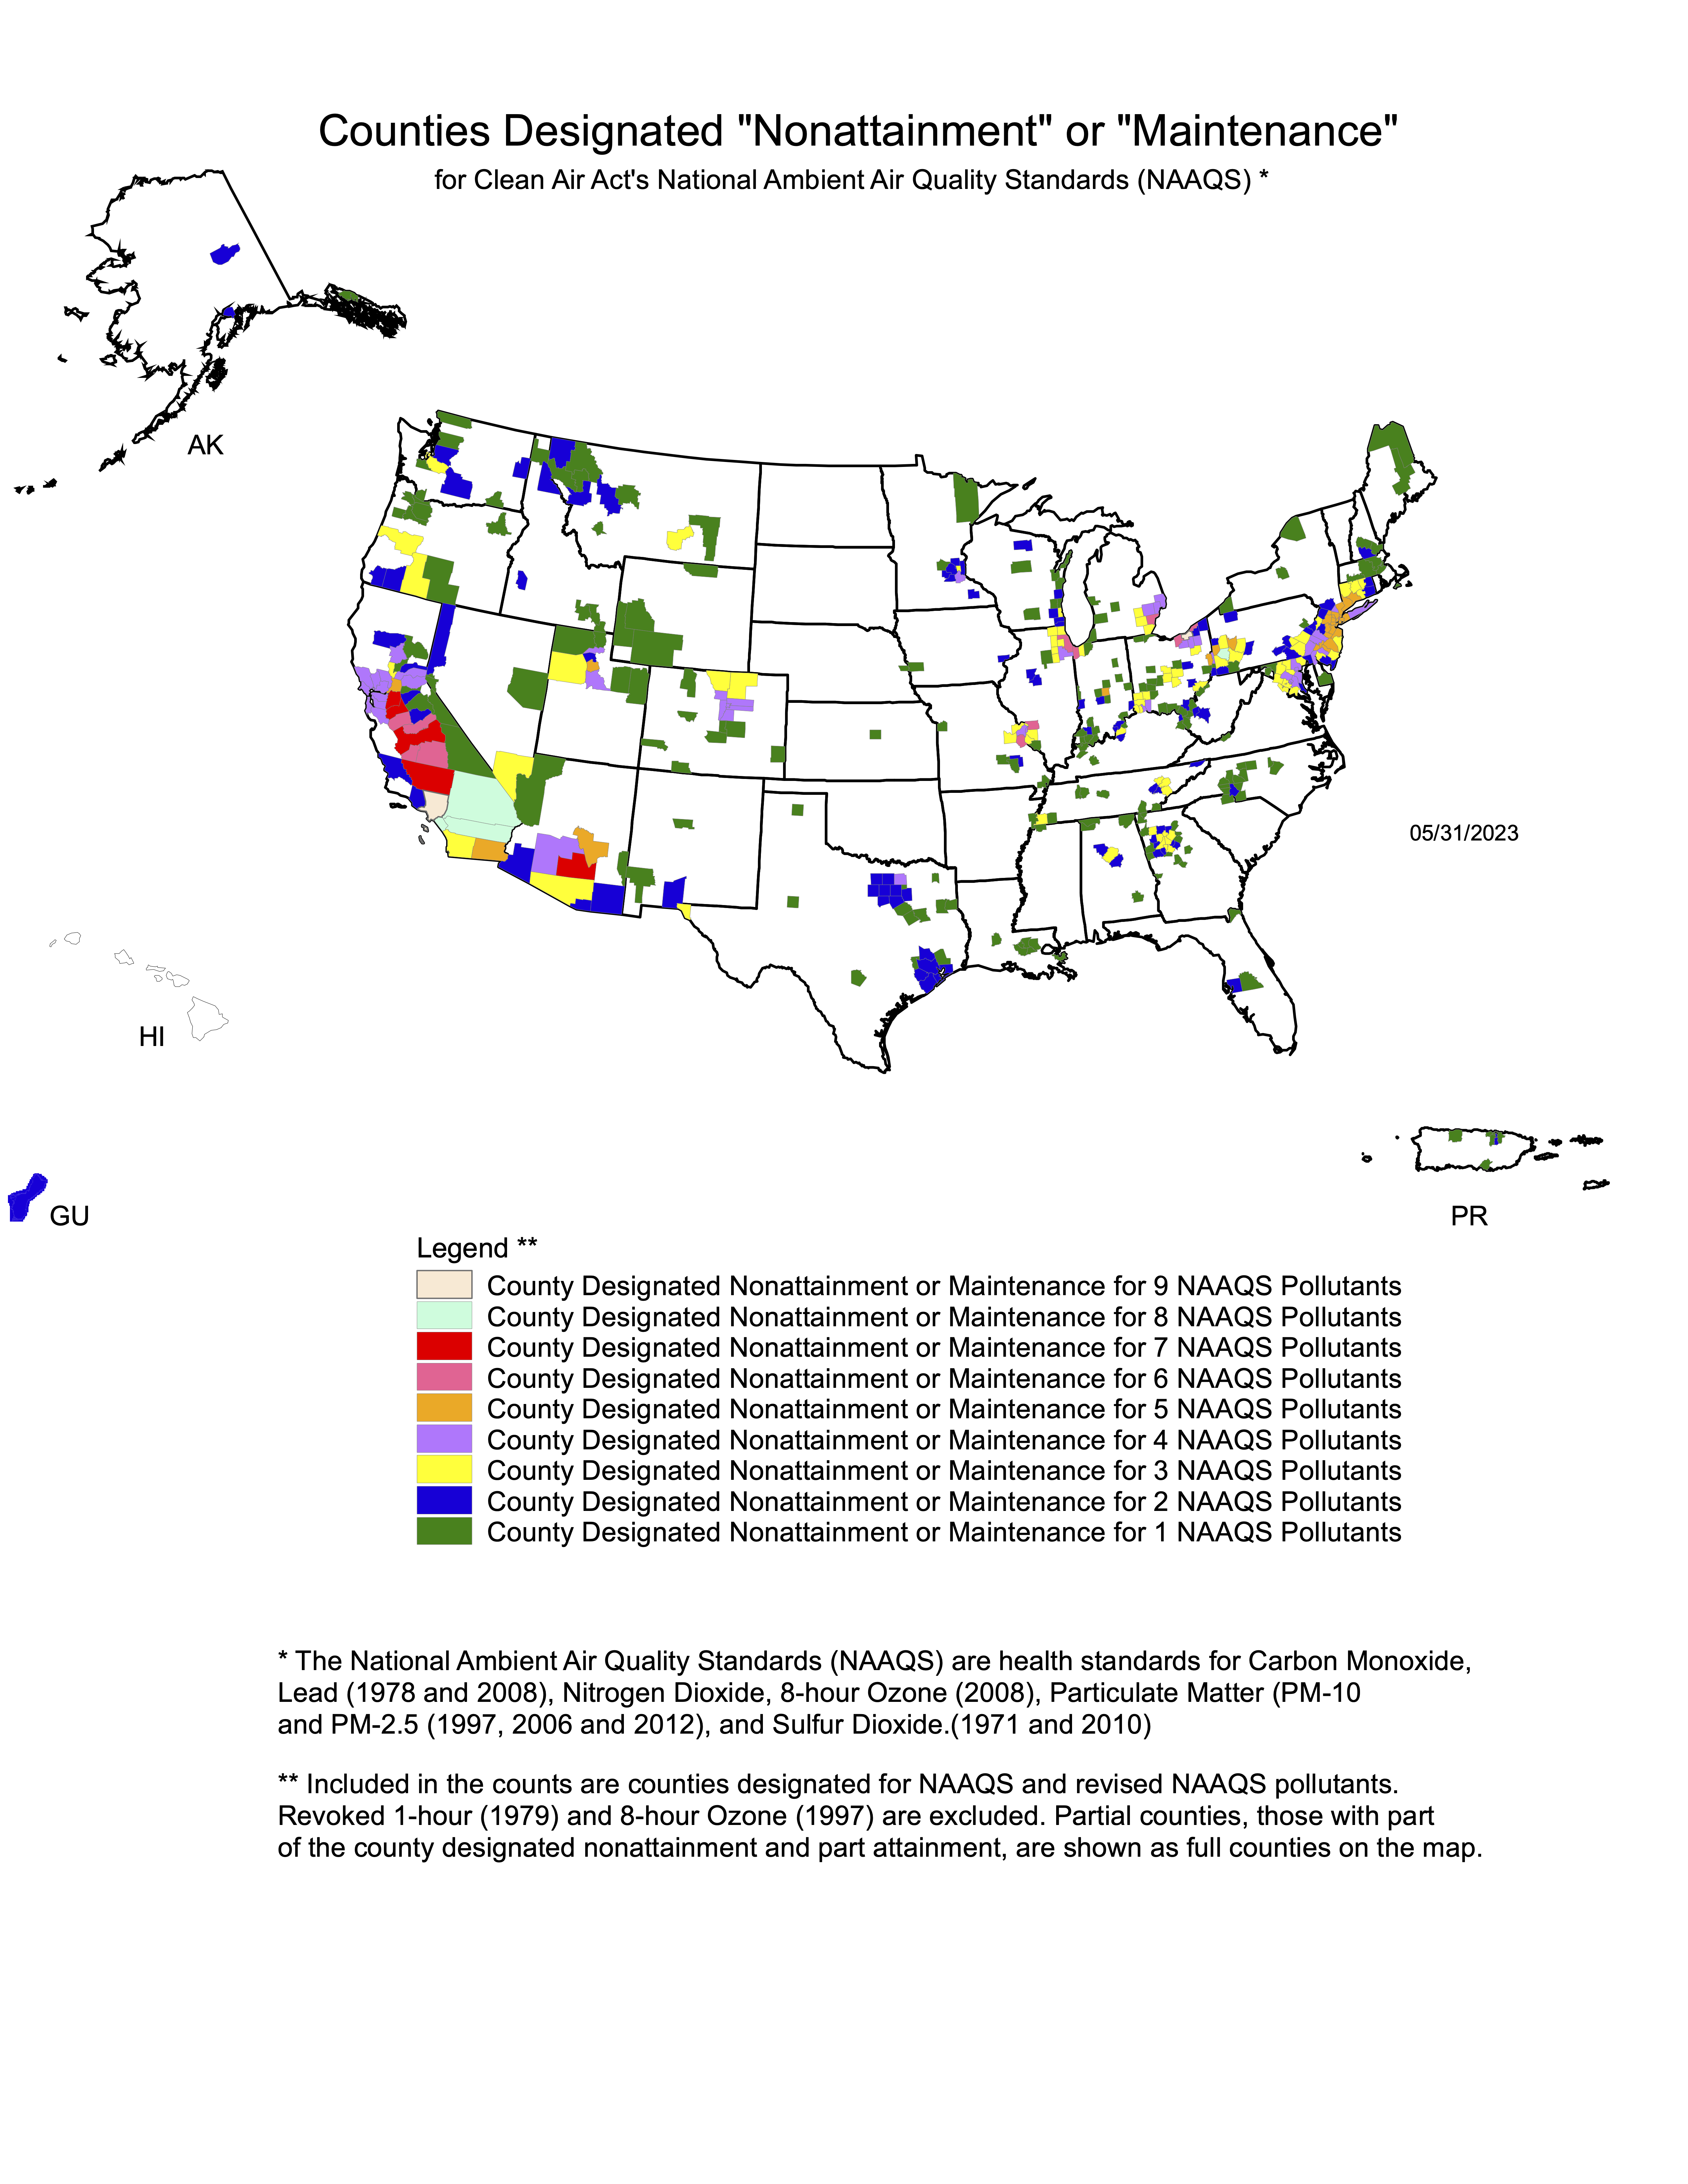
\includegraphics[width=6in,height=\textheight]{images/mapnmpoll.png}

}

\caption{\label{fig-nonattainment}Nonattainment counties in the United
States, identified by how many criteria pollutants are in
nonattainment.}

\end{figure}

One problem with fine particulate matter and vehicle pollution is that
it has differential effects related to demographics, with some
communities experiencing more severe health disparities (Chakraborty,
2022). In order to more equitably address some of these pollution
problems, the EPA has established guidance related to Environmental
Justice to ``determine any disproportionately high and adverse human
health or environmental effects to low-income, minority, and tribal
populations''. This guidance is met through the National Environmental
Policy Act (NEPA), which requires an impact assessment for every federal
action -- including most transportation infrastructure projects -- that
could have an impact on the environment. A report describing any
potential environmental or health impacts or findings of no significant
impact must be submitted. This process and legislation is intended to
protect communities that could be more adversely affected by new
transportation projects or improvements.

In some ways these national and state measures have helped, and recent
evidence that shows a decrease in air pollution related deaths in the
U.S. (Choma et al., 2021). However, more work needs to be done in order
to further decrease pollution related death and disease. This is true
for existing facilities that can be improved to be more equitable and
less polluted as well as any new policies or projects that can be
designed to limit or decrease pollution.

\hypertarget{active-transportation}{%
\subsection{Active Transportation}\label{active-transportation}}

Active transportation is an intersection of public health and
transportation that includes walking and biking improvements, as well as
public transportation. Both individual activity and public
transportation system design are important when looking at active
transportation. When looking at individual activity, direct correlations
have been found between perceptions of well-being and social contact
which comes through walking and biking and in relation to public
transportation infrastructure a positive correlation was found between
quality of life and multimodal trips Gerike et al. (2019). In addition,
correlations have been found between mode choice, the use of public
transportation, and health, showing that the more a car was used for
transport, the higher the BMI (Body Mass Index), supporting the
connection between health and active transport and support- ing the
improvement of public transportation infrastructure to encourage
sustainable mobility Dons et al. (2018).

Active transportation measures and how they impact health can be
somewhat difficult to track, but the best way to do so is by analyzing
different data that has been collected in regards to health and
transportation. To analyze the data on active transportation more
completely, the US Department of Transportation (2022) has partnered
with the Centers for Disease Control and Prevention (CDC) to develop the
Transportation and Health Tool. This tool provides easy access to data
of public health indicators and transportation in each US State and
metropolitan area. These data include indicators such as obesity rates,
percent of physical activity in trips taken, and how much federal
funding was used to support active transportation infrastructure.

Using this data from 2017 in each state we created the maps show in
Figure~\ref{fig-obeseactivity}. Figure~\ref{fig-obeseactivity} (A) shows
the obesity rates by state with 24.2\% being the least in Colorado while
(B) shows the estimated percent of trips that include physical activity
(walking, bicycling, and walk-access public transport). As can be seen
there does seem to be some pattern, with those states that have a higher
physical activity, also having a lower obesity rate. There are a few
outliers, such as Nevada, with a low obesity rate and a low physical
activity percentage, but overall, there is a correlation coefficient
between the two indicators of 0.64. It should be noted in this context
that obesity is a complex disease with many contributing factors, of
which physical activity is only one (Dhurandhar et al., 2021).

\begin{figure}

\begin{minipage}[t]{0.50\linewidth}

{\centering 

\raisebox{-\height}{

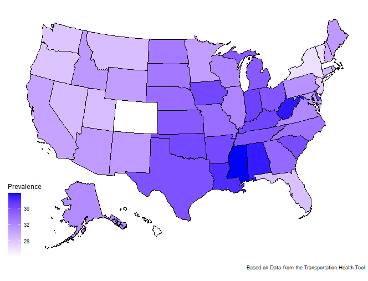
\includegraphics[width=3in,height=\textheight]{images/obesityrates.png}

}

}

\subcaption{\label{fig-obeseactivity-1}Obesity}
\end{minipage}%
%
\begin{minipage}[t]{0.50\linewidth}

{\centering 

\raisebox{-\height}{

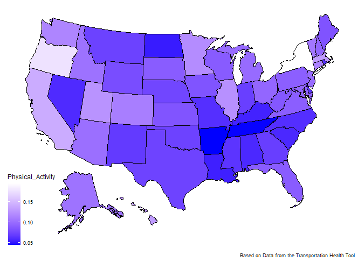
\includegraphics[width=3in,height=\textheight]{images/physicalactivityrates.png}

}

}

\subcaption{\label{fig-obeseactivity-2}Physical Activity}
\end{minipage}%

\caption{\label{fig-obeseactivity}State-level rates of obesity and
physical activity of trips.}

\end{figure}

Obesity is a problem in the United States, and with these graphs there
does seem to be a correlation between increased active transportation
and decreased obesity. In order to improve public health one goal could
be to improve physical activity in transportation dramatically in
states. The highest percentage of physical activity was in New York with
about 20\%. In order to improve this percentage to make 20\% be a more
normal value rather than the exception it is important that each state
put more of an emphasis on public transportation and active
transportation projects.

\hypertarget{accessibility-to-resources}{%
\subsection{Accessibility to
Resources}\label{accessibility-to-resources}}

In addition to helping improve health, public transportation and active
transportation project also improve accessibility to resources.
Accessibility to resources has also been widely studied in the past and
will be analyzed more completely later in this chapter. The main idea of
equitable accessibility is to make sure that each race, economic
background, and age has an equal transportation option or alternative to
access different public goods and resources. Equitable accessibility can
have a dramatic impact on public health and is an important part of
transportation policy (Aggarwal et al., 2014). However, the presence of
accessibility to resources in research and application in different
states is somewhat limited.

At a minimum each state must adhere to the federal Americans with
Disabilities Act (ADA) standard when designing roadways or other
infrastructure. In addition, there is the federal complete streets
policy that is implemented throughout the nation. According to Smart
Growth America (2023), a non-profit organization that helps foster
equitable and sustainable communities, there are 35 state governments
that have adopted complete streets policies, with Utah being one of
those states. Complete Streets requires streets to be planned, designed,
and maintained to enable safe and comfortable access and travel for all
users regardless of age, abilities and mode of transportation.

\begin{figure}[t]

{\centering 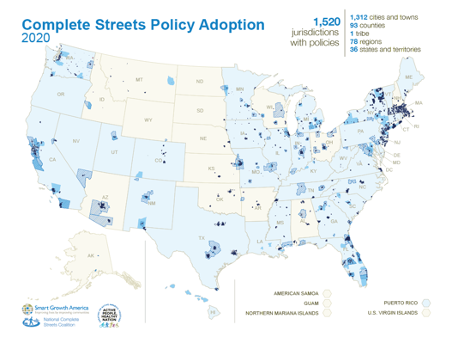
\includegraphics[width=6in,height=\textheight]{images/completestreets.png}

}

\caption{\label{fig-completestreets}Jurisdictions with complete streets
policies in the United States.}

\end{figure}

This map shown in Figure~\ref{fig-completestreets} gives a visual
representation of which counties, cities, and towns have adopted a
complete streets policy. As can be seen, even in the states that have
adopted a policy, there are still massive regions that do not have that
policy implemented that still need the impact of equitable accessibility
in projects and policy.

\hypertarget{access-to-nutrition}{%
\section{Access to Nutrition}\label{access-to-nutrition}}

\hypertarget{access-and-equity}{%
\subsection{Access and Equity}\label{access-and-equity}}

Equitable access to community resources has been a topic of research and
study, especially when looking at the impacts on measures of well-being
and economic opportunity. Current social issues, economic opportunity
and equity are significant topics that can help us ensure that each
population demographic can have similar opportunities. Equity as a term
is being fair and impartial, different from equality. Equality is
providing the exact same thing to all people, whereas equity would
provide different things to different people because of their
circumstances in order to create a fair system. Lower-income populations
frequently sit at a different level of advantage than higher-income
populations, including when looking at accessibility Witten et al.
(2003). It is important to discover how different transportation
policies can improve accessibility to create better equity. Creating
equitable societies and equitable transportation policies is important
in order to remove any discrimination already present in the
transportation network. In this way states can decrease the disparity
that is common when looking at different neighborhoods and demographics.
Perhaps there are low-income neighborhoods that do not have the same
economic opportunity or resource accessibility as high-income
neighborhoods. If we increase the accessibility of low-income
neighborhoods, could that then increase the quality of life and health
for those neighborhoods as well?

In addition to economic opportunity, the connection between well-being
and opportunity is also significant, discovering who has access to which
resources and how that access corresponds to their health Schwanen et
al. (2015). A subjective sense of positive well-being correlates with
increased access to more community resources: increased access was
specifically connected with variety of resources, not necessarily number
of the same type of resource. This increased access is true for both
high- and low-income populations. However, high-income demographics
frequently tend have better access to a variety of resources because of
such variables as available child care, a transportation source
available, or even time available to do things Liu et al. (2022) . In
addition, increased access to resources such as parks or other
greenspace have been found to decrease likelihood of mental health
disorders, as well as improve physical activity Madzia et al. (2019).
Different age groups each have a different response to access to
greenspace. However, among all age groups there is a positive
correlation.In addition to health impacts, lack of accessibility also
affects economic opportunity when considering access to employment,
affordable care, and other stores and shops Hu (2015).

\hypertarget{food-deserts-and-swamps}{%
\subsection{Food Deserts and Swamps}\label{food-deserts-and-swamps}}

While there are many different community resources that can be the
center of study, such as libraries, green space, hospitals, etc., this
project will focus on the resource of grocery stores and discovering any
correlation between accessibility to good nutrition environments such as
healthy grocery stores and the demographic makeup of specific block
groups, such as economic bracket and different ethnic groups. Lack of
accessibility to grocery stores can have an effect on physical health
and well-being (Aggarwal et al., 2014). This access is related directly
with consumption of healthy foods, as well as indirectly with perceived
sense of well-being.

Much of the current research that has been done has shown a different
level of accessibility for different demographics, such as low income
populations. Low income populations have been shown to frequently have
less access to fresh fruits and vegetables Losada-Rojas et al. (2021).
This may not be directly correlated to the physical distance from a
grocery store, but the store that was chosen for these demographics. In
a study analyzing grocery store choice in Seattle it was found that in
some instances, there is a closer store with better produce, but for
some reason it was not chosen and instead a store that was further away
was chosen that did not have the same quantity and variety of fresh
produce. This was found again in a different study, that frequently
people will travel to a store that is not the closest store for
different reasons Hillier et al. (2011). This study will help to
determine that choice pattern and identify which variables are important
when choosing a store to help improve accessibility more than simple
distance measures.

However, areas that do not have any full service grocery stores however
are also important to look at, with those areas being known as food
swamps. These food swamps are an idea that there are locations where
there is not healthy food available, so the only option that is readily
accessible for food or meals would be fast food or convenience stores.
There have been studies analyzing the different food swamp areas and
what could be done to improve those areas, such as adding grocery stores
or corner markets (Bao et al., 2020). These food swamps are areas that
discriminate between those without readily available transit options and
those with easy access to cars, creating a barrier to equity. In
addition, these food swamp areas are especially significant when looking
at the public health impacts of food accessibility and discovering how
we can improve the quality of food available to those in every
demographic to create an equitable solution to health differences.

Past research done clearly shows that location of store, quality of
store, and price of store all have an impact on choice of grocery store
and accessibility to grocery stores. This impacts the quality of life
and overall health and well-being of individuals and shows the
importance of discovering which variables are most significant in
grocery store choice in order to improve accessibility and equity. What
much existing research suffers from, however, is the wide variety of
measures of access and the definitions used to describe a ``grocery
store.'' Certainly convenience stores do not typically provide the same
variety and quality of goods, but simply excluding them from analyses
ignores how many people obtain a large share of their daily and weekly
nutrition, for better or worse. A measure that can incorporate
multimodal access to stores as well as qualitatively describe the stores
along a continuous array of measures is desirable.

\bookmarksetup{startatroot}

\hypertarget{sec-methods}{%
\chapter{Methods}\label{sec-methods}}

This section describes how we construct a model of access to grocery
stores in communities in Utah. We first describe the theoretical model,
and then describe data collection efforts to estimate this model and
apply it.

\hypertarget{model}{%
\section{Model}\label{model}}

A typical model of destination choice (Recker and Kostyniuk, 1978) can
be described as a random utility maximization model where the utility of
an individual \(i\) choosing a particular destination \(j\) is
\begin{equation}\protect\hypertarget{eq-utility}{}{ U_{ij} = \beta_{s}f(k_{ij}) + \beta_{x}(X_j) }\label{eq-utility}\end{equation}
where \(f(k_{ij})\) is a function of the travel impedance or costs from
\(i\) to \(j\) and \(X_{j}\) represents the location attributes of
\(j\). The coefficients \(\beta\) can be estimated given sufficient data
revealing the choices of individuals. The probability that individual at
location \(i\) will choose alternative \(j\) from a choice set \(J\) can
be estimated with a multinomial logit model (MNL) (McFadden, 1974),
\begin{equation}\protect\hypertarget{eq-mnl}{}{ P_i(j) = \frac{\exp(U_{ij})}{\sum_{j' \in J}{\exp(U_{ij'})}}}\label{eq-mnl}\end{equation}
The overall fit of the model can be described with the Akaike
Information Criterion (AIC) --- which should be minimized --- or by the
McFadden likelihood ratio
\(\rho^2_0 = 1 - \ln\mathcal{L} / \ln\mathcal{L}_0\). In this ratio
\(\ln{\mathcal{L}}\) is the model log-likelihood and
\(\ln{\mathcal{L}_0}\) the log-likelihood of an alternative model where
all destinations are equally likely; a higher \(\rho^2_0\) value
indicates more explanatory power relative to this null, random chance
only model.

The idea of using destination choice logsums as accessibility terms is
not new, and the theory for doing so is described in Ben-Akiva and
Lerman (1985, p. 301). Effectively, the natural logarithm of the
denominator in Equation~\ref{eq-mnl} represents the consumer surplus ---
or total benefit --- available to person \(i\):

\begin{equation}\protect\hypertarget{eq-cs}{}{ CS_i = \ln\left(\sum_{j \in J} \exp(U_{ij})\right)}\label{eq-cs}\end{equation}

A difference in logsum measures may exist for a number of reasons that
affect the utility functions described in Equation~\ref{eq-utility}. For
example, individuals at different locations or with different mobility
will see different impedance values \(k_{ij}\) and therefore affected
utility. Changes to the attributes of the destinations \(X_j\) will
likewise affect the utility.

Despite the relative maturity of this theory, applications of
utility-based access in the literature are still rare, outside of public
transport forecasting analyses (Geurs et al., 2010). The rarity is
likely explained by an unfamiliarity with destination choice models and
the ready availability of simpler methods on one hand (Logan et al.,
2019), and the difficulty in obtaining a suitable estimation dataset for
particular land uses on the other (Kaczynski et al., 2016). This second
limitation has been somewhat improved by a new methodology developed by
Macfarlane et al. (2022) , relying on commercial location-based services
data to estimate the affinity for simulated agents to visit destinations
of varying attributes and distances.

\hypertarget{data}{%
\section{Data}\label{data}}

In this research, we develop a unique dataset to estimate the
destination choice utility coefficients for grocery store choice in
three different communities in Utah. The three communities were selected
to maximize potential observed differences in utility between community
residents. The three communities are Utah County, West Salt Lake Valley,
and San Juan County. Note that in this document we refer to the second
community as ``Salt Lake'' even though this does not refer to the entire
Salt Lake County nor to Salt Lake City, rather, we focus on communities
in the western part of the valley, such as Magna, Kearns, and West
Valley City.

Table~\ref{tbl-acsdata} shows several key population statistics based on
2021 American Community Survey data for block groups in the three
communities of interest. Utah County is a largely suburban county with
high incomes and a low percentage of minority individuals. The Salt Lake
region is more dense with somewhat lower incomes and household sizes but
a high share of minority individuals. San Juan County is primarily
rural, with a few small communities and a large reservation for the
Navajo Tribe.

\hypertarget{tbl-acsdata}{}
\begin{table}
\caption{\label{tbl-acsdata}Demographic Statistics of Study Region }\tabularnewline

\centering
\begin{tabular}[t]{lrrr}
\toprule
 & Utah & Salt Lake & San Juan\\
\midrule
Total population & 627,098 & 655,830 & 7,091\\
Total households & 171,538 & 216,731 & 2,090\\
Housing units per sq. km & 599 & 831 & 103\\
Median income & 79,453 & 64,868 & 58,586\\
Percent minority individuals & 18 & 36 & 26\\
\bottomrule
\end{tabular}
\end{table}

Estimating the utility model described in Equation~\ref{eq-mnl} for
grocery stores requires three interrelated data elements:

\begin{enumerate}
\def\labelenumi{\arabic{enumi}.}
\tightlist
\item
  an inventory of grocery store attributes \(X_j\),
\item
  a representative travel impedance matrix \(K\) composed of all
  combinations of origin \(i\) and destination \(j\).
\item
  a database of observed person flows between \(i\) and \(j\) by which
  to estimate the \(\beta\) coefficients.
\end{enumerate}

We describe each of these elements in turn in the following sections.

\hypertarget{store-attributes}{%
\subsection{Store Attributes}\label{store-attributes}}

The store attributes were collected using the Nutritional Environment
Measures Survey --- Stores (NEMS-S) tool (Glanz et al., 2007). This tool
was developed to reveal significant differences in the availability and
cost of healthy foods in an environment, and has been validated for this
purpose. Beyond superficial attributes such as the store category
(dollar store, convenience store, ethnic market, etc.) and the number of
registers, the NEMS-S collects detailed information about numerous store
offerings such as the availability of produce, dairy products, lean
meats, juices, and canned and dry goods of various specific types. Of
particular interest to the survey are availability and price
differentials of lower-fat alternatives: for example, the survey
instrument requests the shelf space allocated to milk products of
various fat levels and the price of each product.

Student research assistants collected the store attributes by visiting
grocery stores, dollar stores, ethnic markets, and other food markets in
the three communities of interest described above. Stores were
identified using internet-based maps combined with in-person validation
and observation. The student researchers completed the NEMS-S instrument
with the aid of a digital survey and a tablet computer. Each researcher
who collected data was trained to use the survey at a control store in
Provo, and the training data helped to eliminate the risk of surveyor
bias. The store attributes were collected in the spring of 2021 for Utah
County and spring of 2022 for Salt Lake and San Juan Counties. In Utah
and Salt Lake Counties, we included dollar stores and grocery stores but
did not include convenience stores. Given the rural nature of San Juan
County, we made two adjustments to capture the entirety of the nutrition
environment. First, we included convenience stores and trading posts if
they were the only food market in a community. We also included
full-service grocery stores in Cortez, Colorado, and Farmington, New
Mexico in the San Juan data collection, as community conversations made
it clear that many residents will drive these long distances for
periodic shopping with greater availability and lower prices.

Using the information in the NEMS-S survey, two measures of a store can
be calculated: an availability score based on whether stores stock
particular items as well as lower-calorie options; and a cost score
describing the spread between prices of these options. These score
values are described in Lunsford et al. (2021), and we developed an R
package to compute the scores; this package is available at
\url{https://github.com/byu-transpolab/nemsr}. In the availability score
each store is given a value for whether or not there are more healthful
options available in the store, such as low-calorie chips, or low-fat
milk. If the store does not have a more healthful option in a category
it receives a lower score, so stores with more availability of healthful
food options will receive a higher availability score. For the cost
score, the measure is the price spread between healthful and less
healful options: if the price of whole wheat bread is cheaper than white
bread, the store receives positive points for the cost option, if the
price is the same then zero points are awarded, and if the wheat bread
is more expensive then the store receives negative points. Thus a store
with a higher availability and cost score will have both more healthful
options, and a more advantageous pricing scheme towards those options.

One important store attribute that the NEMS-S instrument does not
collect or compute directly is a measure of the cost of common goods
that can be compared across stores. We therefore used the data collected
from the NEMS-S instrument to construct a market basket-based
affordability measure that could be compared across stores, following
the approach of Hedrick et al. (2022). This market basket score is based
on the US Department of Agriculture (USDA) 2021 Thrifty Food Plan (FNS,
2021), which calculates a reference market basket for a family of four.
Because this market basket contains more (and sometimes different) items
than what the NEMS-S instrument requests, we chose relevant items from
our NEMS-S data as replacements. For example, the USDA market basket
contains a certain amount of poultry, but the NEMS-S score collects the
per-pound cost of ground beef at various fat contents. For any stores
that were missing any of the elements in the market basket, we first
substituted with another ingredient that would fit the nutritional
requirements. If no substitute was available, we included the average
price of the missing good at other stores in that community multiplied
by 1.5 as a penalty for not containing the product. The final market
basket score is the total cost of all foods in the market basket. These
costs can then be compared from store to store to understand general
affordability comparisons between stores.

\hypertarget{tbl-nems}{}
\begin{table}
\caption{\label{tbl-nems}Grocery Store Attributes }\tabularnewline

\centering
\resizebox{\linewidth}{!}{
\begin{tabular}[t]{llrrrrrr}
\toprule
\multicolumn{2}{c}{ } & \multicolumn{2}{c}{Utah (N=63)} & \multicolumn{2}{c}{Salt Lake (N=39)} & \multicolumn{2}{c}{San Juan (N=50)} \\
\cmidrule(l{3pt}r{3pt}){3-4} \cmidrule(l{3pt}r{3pt}){5-6} \cmidrule(l{3pt}r{3pt}){7-8}
  &    & Mean & Std. Dev. & Mean & Std. Dev. & Mean & Std. Dev.\\
\midrule
Registers (incl. self checkout) &  & 12.5 & 11.7 & 9.9 & 8.9 & 6.1 & 8.8\\
NEMS-S availability score &  & 18.7 & 8.4 & 16.2 & 8.1 & 13.2 & 7.6\\
NEMS-S cost score &  & 1.9 & 2.3 & 2.3 & 2.2 & 1.9 & 1.9\\
Market basket cost &  & 126.1 & 21.5 & 141.6 & 19.2 & 157.6 & 16.8\\
\midrule
 &  & N & Pct. & N & Pct. & N & Pct.\\
Type & Convenience Store & 2 & 3.2 & 0 & 0.0 & 10 & 20.0\\
 & Dollar Store & 5 & 7.9 & 11 & 28.2 & 15 & 30.0\\
 & Grocery Store & 50 & 79.4 & 27 & 69.2 & 19 & 38.0\\
 & Other & 6 & 9.5 & 1 & 2.6 & 6 & 12.0\\
Pharmacy & FALSE & 42 & 66.7 & 32 & 82.1 & 43 & 86.0\\
 & TRUE & 21 & 33.3 & 7 & 17.9 & 7 & 14.0\\
Ethnic market & FALSE & 55 & 87.3 & 30 & 76.9 & 47 & 94.0\\
 & TRUE & 8 & 12.7 & 9 & 23.1 & 3 & 6.0\\
Other merchandise sold & FALSE & 52 & 82.5 & 35 & 89.7 & 47 & 94.0\\
 & TRUE & 11 & 17.5 & 4 & 10.3 & 3 & 6.0\\
\bottomrule
\end{tabular}}
\end{table}

Table~\ref{tbl-nems} presents the store attribute data collected for
each community. Utah County generally has the largest average store size
(as measured by the number of checkout registers) while having the
lowest market basket cost, the highest availability of health food (the
NEMS-S availability score) and the lowest difference between healthy and
unhealthy food (the NEMS-S cost score). San Juan County has the smallest
average stores, highest costs and the lowest availability of healthy
options, and Salt Lake falls in between.

\hypertarget{imputation-of-missing-store-data}{%
\subsection{Imputation of Missing Store
Data}\label{imputation-of-missing-store-data}}

We collected detailed store attributes for stores in Utah County, San
Juan County, and a portion of Salt Lake County using the NEMS-S survey
instrument. These attributes form the basis of the choice models used to
determine access, but understanding access in other parts of Salt Lake
City or the state of Utah requires us to impute the attributes onto the
stores that we did not collect.

To do this, we used web-based mapping databases (including OpenStreetMap
and Google Maps) to obtain a list of grocery stores, dollar stores, and
appropriate convenience stores throughout the state. From this search,
we were able to determine each store's location, brand name, and store
type, which we also collected in the manual data assembly efforts. Using
this information, we built a multiple imputation model using the
\texttt{mice} package for R (van Buuren and Groothuis-Oudshoorn, 2011).
The predictor variables in the imputation included the store brand and
type, as well as the average income and housing density in the nine
closest block groups to the store location (based on population-weighted
centroids).

\begin{figure}[t]

{\centering 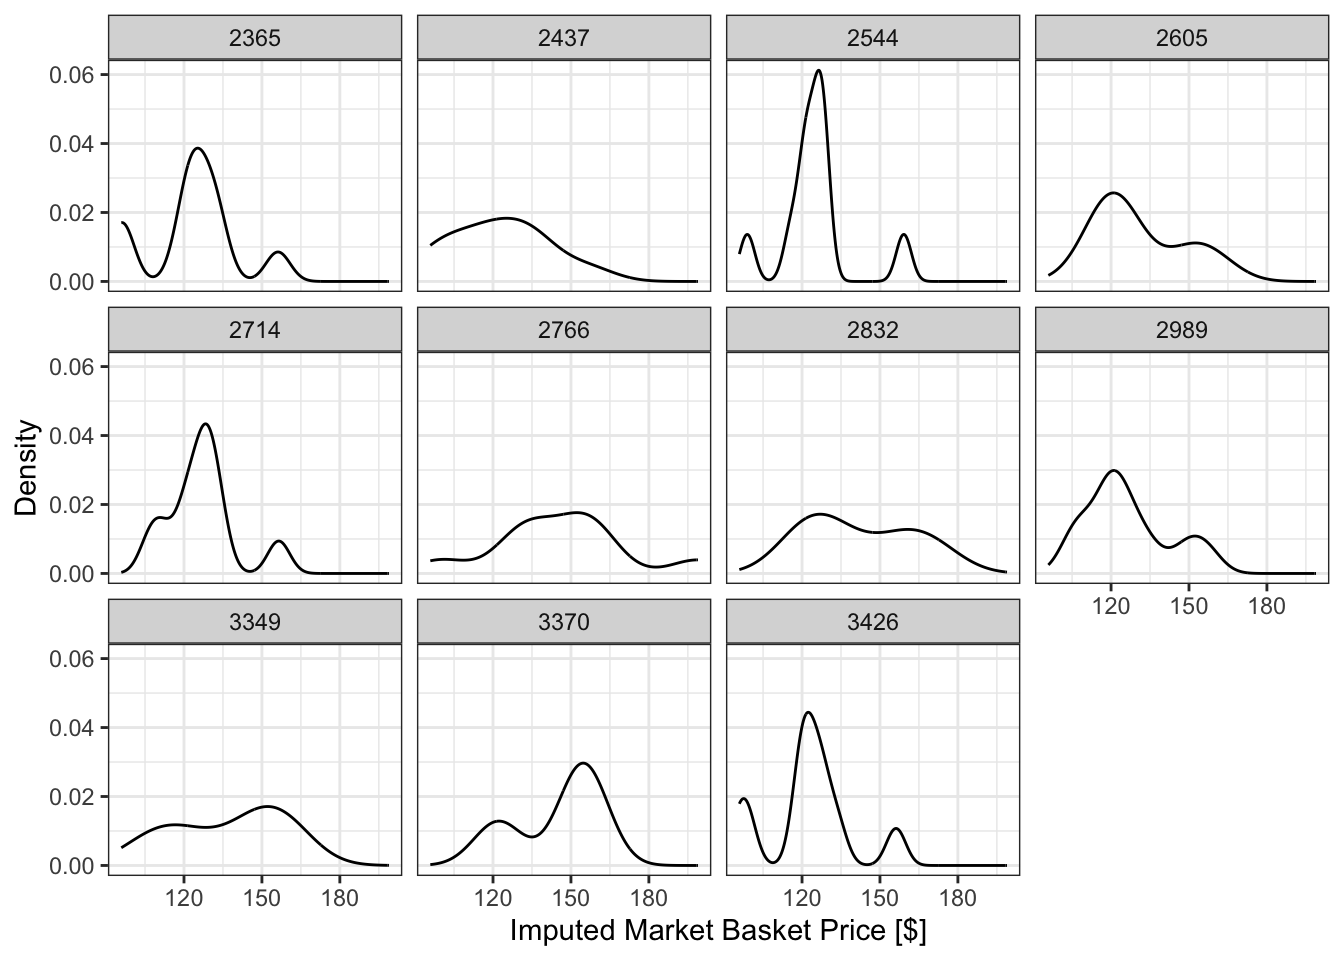
\includegraphics[width=5in,height=\textheight]{03_methods_files/figure-pdf/fig-marketimp-1.pdf}

}

\caption{\label{fig-marketimp}Imputed market price values for 15 random
grocery stores.}

\end{figure}

Thirty iterations of the multiple imputation algorithm were run for each
of ten independent imputations. Figure~\ref{fig-marketimp} shows the
density of the ten imputed market basket prices for a randomly selected
set of 15 stores. As the figure reveals, there is some general peaking
in the predicted market price for most stores, but the imputation model
still predicts a wide range of possible prices for most stores. When
using the imputed data for analysis, we take the mean of the ten
predictions for continuous values, and the mode for discrete values.

\hypertarget{sec-mcls}{%
\subsection{Travel Impedances}\label{sec-mcls}}

The second element of the utility equation in Equation~\ref{eq-utility}
is the travel impedance between \(i\) and \(j\). Many possibilities for
representing this impedance exist, from basic euclidean distance to
complex network paths. A primary purpose of the model we are developing
in this research is to study comparative tradeoffs between
infrastructure-focused and environment-focused improvements to the
nutrition access of households. It is therefore essential that we use a
travel impedance measure that can combine and compare the cost of
traveling by multiple modes so that highway improvements and transit /
active transport improvements can be compared in the same basic model.

Just as the log-sum of a destination choice model is a measure that sums
the utility of multiple destination attributes and costs in a rigorous
manner, the log-sum of a mode choice model combines the utilities of all
available travel modes. In this study we assert the following mode
choice utility equations: \begin{align*} 
  V_{\mathrm{auto}, ij} &= -0.028(t_{\mathrm{auto}, ij})\\
  V_{\mathrm{bus}, ij} &= -4 -0.028(t_{\mathrm{bus}, ij}) -0.056(t_{\mathrm{wait}, ij}) -0.056(t_{\mathrm{access}, ij})\\
  V_{\mathrm{walk, ij}} &= -5 -0.028(t_{\mathrm{walk}, ij}) -1.116(d_{ij<1.5}) -5.58(d_{ij>1.5})\\
\end{align*} where \(t\) is the in-vehicle travel time in minutes for
each mode between \(i\) and \(j\). The transit utility function
additionally includes the wait time for transit as well as the time
necessary to access the transit mode on both ends by walking. The walk
utility includes a per-mile distance disutility that increases for
distances greater than 1.5 miles. These equations and coefficients are
adapted from a statewide mode choice model developed for UDOT research
(Barnes, 2021).

The log-sum, or total weighted impedance by all modes is therefore
\begin{equation}\protect\hypertarget{eq-mcls}{}{
k_{ij} = \ln(e^{V_{\mathrm{auto}, ij}} + e^{V_{\mathrm{bus}, ij}} + e^{V_{\mathrm{walk},ij}})
}\label{eq-mcls}\end{equation}

In this implementation, \(i\) is the population-weighted centroid of a
2020 Census block group, and \(j\) is an individual grocery store. We
measure the travel times from each \(i\) to each \(j\) using the
\texttt{r5r} implementation of the R5 routing engine (Conway et al.,
2018, 2017; Conway and Stewart, 2019; Pereira et al., 2021). This
algorithm uses common data elements --- OpenStreetMap roadway and active
transport networks alongside General Transit Feed Specification (GTFS)
transit service files --- to simulate multiple realistic route options
by all requested modes. We obtained OpenStreetMap networks and the Utah
Transit Authority GTFS file valid for May 2023 and requested the minimum
total travel time by each mode of auto, transit, and walking for a
departure between 8 AM and 9 AM on May 10, 2023. The total allowable
trip time by any mode was set to 120 minutes, and the walk distance was
capped at 10 kilometers; if a particular \(i,j\) pair exceeded these
parameters then the mode was presumed to not be available and
contributes no utility to the log-sum.

\hypertarget{mobile-device-data}{%
\subsection{Mobile Device Data}\label{mobile-device-data}}

The final element of destination utility presented in
Equation~\ref{eq-utility} are the coefficients, which are often
estimated from household travel surveys in a travel demand context. It
is unlikely, however, that typical household diaries would include
enough trips to grocery stores and similar destinations to create a
representative sample.

Emerging mobile device data, however, could reveal the typical home
locations for people who are observed in the space of a particular
store. Macfarlane et al. (2022) present a method for estimating
destination choice models from such data, which we repeat in this study.
We provided a set of geometric polygons for the grocery stores of
interest to StreetLight Data, Inc., a commercial location-based services
aggregator and reseller. StreetLight Data in turn provided data on the
number of mobile devices observed in each polygon grouped by the
inferred residence block group of those devices during summer 2022. We
then created a simulated destination choice estimation dataset for each
community resource by sampling 10,000 block group - grocery store
``trips'' from the StreetLight dataset. This created a ``chosen''
alternative; we then sampled ten additional stores from the same
community at random (each simulated trip was paired with a different
sampled store) to serve as the non-chosen alternatives. Random sampling
of alternatives is a common practice that results in unbiased estimates,
though the standard errors of the estimates might be larger than could
be obtained through a more carefully designed sampling scheme (Train,
2009).

\bookmarksetup{startatroot}

\hypertarget{sec-results}{%
\chapter{Results}\label{sec-results}}

This section presents results on the nutrition environment in each of
the three communities of Utah County, West Salt Lake County, and San
Juan County, along with destination choice model estimates and their
application to creating accessibility maps of each community and the
entire state of Utah.

\hypertarget{sec-nems}{%
\section{Nutrition Environment}\label{sec-nems}}

Though some basic descriptive statistics of the grocery store attributes
were presented in Table~\ref{tbl-nems}, some additional exploration of
these attributes is valuable to understand the nutrition environment in
these three communities.

\begin{figure}[t]

{\centering 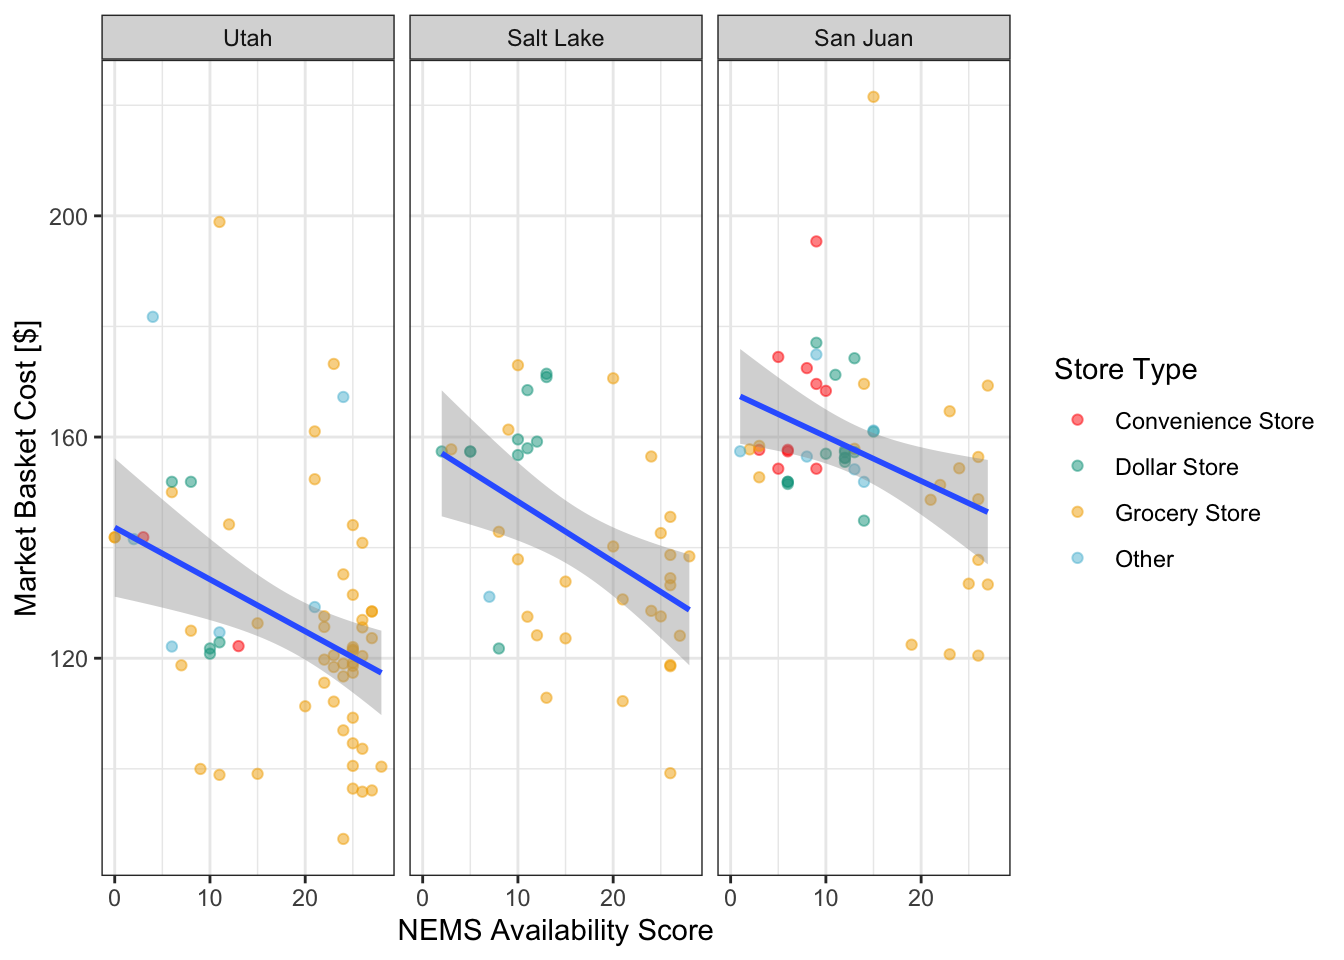
\includegraphics{04_estimation_files/figure-pdf/fig-nems-market-avail-1.pdf}

}

\caption{\label{fig-nems-market-avail}Relationship between NEMS
availability score and market basket score in each study community. Utah
county prices adjusted for 2021-2022 annual inflation.}

\end{figure}

Figure~\ref{fig-nems-market-avail} presents the relationship between the
recorded NEMS availability score and the USDA market basket cost at the
stores by community and store type. In all three communities, the
relationship is strongly negative, with stores that stock more varieties
of goods also having overall lower prices for those goods. This is
emphasized by the bottom-right quadrants of these plots (high
availability, low-cost) being dominated by full-service grocery stores,
which have more availability and lower prices than convenience stores or
dollar stores, but require higher traffic and demand to make up for
their lower profit margins. Average prices in Utah County are lower than
prices in the other two communities across the availability spectrum;
this is true even after adjusting for 9.4\% annual inflation between
March 2021 and March 2022 in food products (Bureau of Labor Statistics,
2023).

\begin{figure}[t]

{\centering 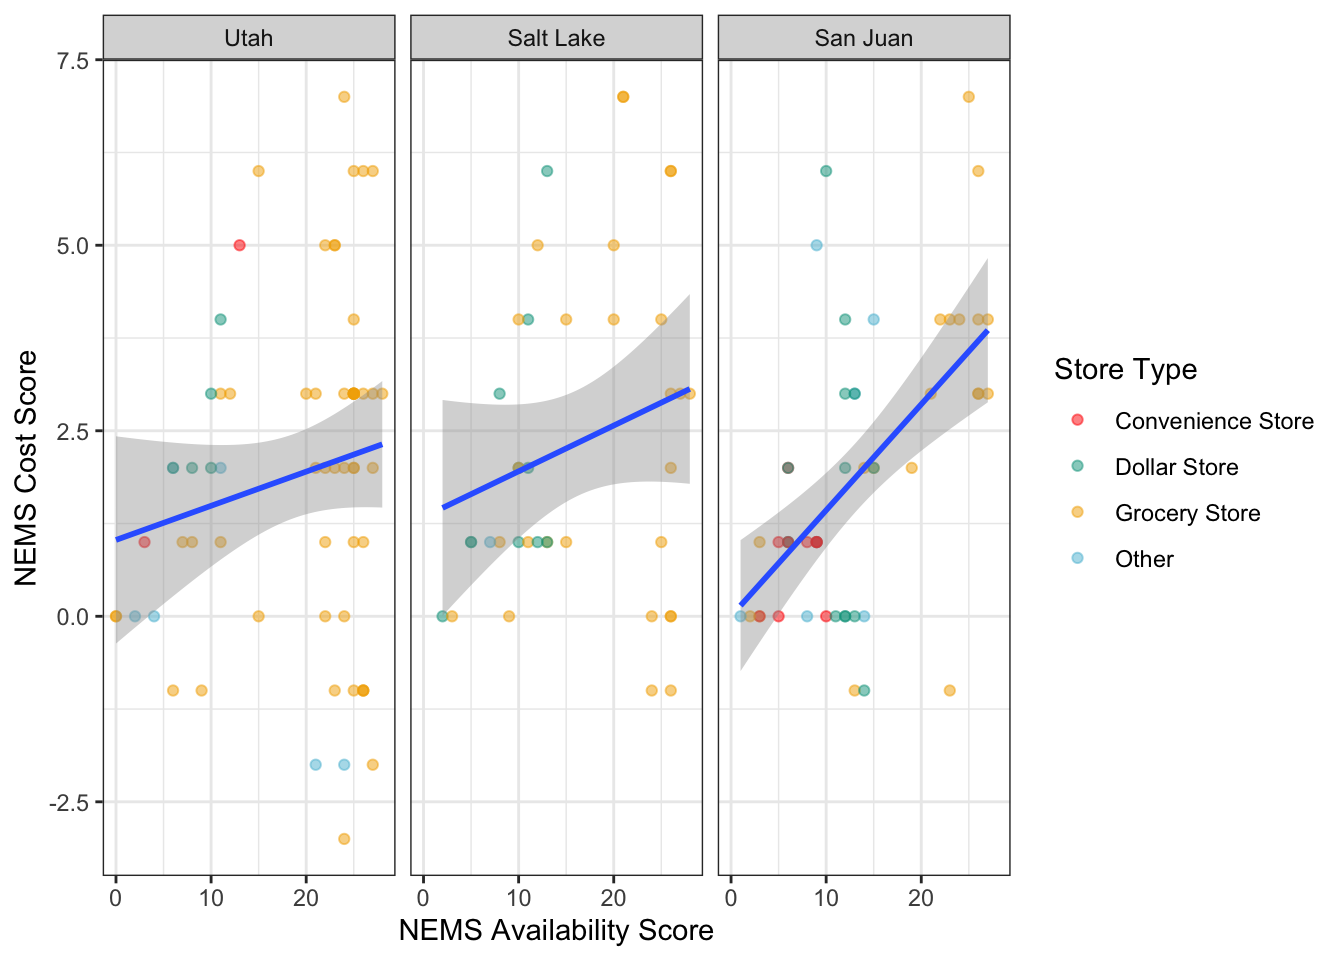
\includegraphics{04_estimation_files/figure-pdf/fig-nems-cost-avail-1.pdf}

}

\caption{\label{fig-nems-cost-avail}Relationship between NEMS
availability score and cost score in each study community.}

\end{figure}

Figure~\ref{fig-nems-cost-avail} shows the relationship between the NEMS
availability and cost scores. In this case the relationship is generally
positive, with stores that stock more healthful options also placing
these options at competitive prices. Conversely, stores with fewer
options tend to place the options they do stock at a higher price point.
This relationship between availability and cost of healthful goods is
strongest in San Juan County, with convenience stores anchoring the
low-availability, high-premium quadrant for healthy food. It should be
noted that these convenience stores also exist in the Utah County
community, but we explicitly included them in the San Juan data
collection as they are the only food markets of any kind in multiple
towns, with dozens of miles separating towns from each other.

\hypertarget{sec-estimation}{%
\section{Destination Choice}\label{sec-estimation}}

Using the data collected and MNL destination choice model as described
in Chapter~\ref{sec-methods}, we estimate a series of model
specifications in each community with the \texttt{mlogit} package for R
(Croissant, 2020). To illustrate the role of different data elements on
destination choice, we develop and estimate four different utility
equations: \begin{align*}
\mathrm{Access} &= \beta_{MCLS}( k_{ij})\\
\mathrm{NEMS} &= \beta_{n-a} (\mathrm{NEMS-Availability}) + \beta_{n-c}\mathrm({NEMS-Cost})\\
\mathrm{Attributes} &= \beta_{mkt} (\mathrm{Market Basket}) + \mathbf{\beta}_{type}(\mathrm{Type})\\
\mathrm{All} &= \mathrm{Access} + \mathrm{NEMS} + \mathrm{Attributes}\\
\end{align*} The Access model includes only the mode choice logsum
described in Equation~\ref{eq-mcls}. The NEMS model includes the NEMS
cost and availability scores describing the goods the store offers,
while the Attributes model contains information that might be more
conventionally available to shoppers including the size, type, and
average prices at the store. As the nutrition environment in each
community contains different types of stores, the specific type
coefficients differ by community. The All model contains all of the
other three sets of estimated coefficients.

\hypertarget{tbl-utah-models}{}
\begin{table}
\caption{\label{tbl-utah-models}Estimated Models of Utah County }\tabularnewline

\centering
\begin{tabular}[t]{lcccc}
\toprule
  & Access & NEMS & Attributes & All\\
\midrule
Mode Choice Log-sum & 8.090** &  &  & 8.592**\\
 & (95.354) &  &  & (87.875)\\
NEMS Availability Score &  & 0.034** &  & -0.010**\\
 &  & (23.136) &  & (-3.191)\\
NEMS Cost Score &  & 0.029** &  & 0.035**\\
 &  & (6.344) &  & (5.075)\\
USDA Market Basket &  &  & -0.007** & -0.008**\\
 &  &  & (-8.943) & (-8.756)\\
Registers &  &  & 0.057** & 0.062**\\
 &  &  & (55.241) & (39.579)\\
Store Type: Dollar Store &  &  & 1.955** & 2.136**\\
 &  &  & (57.226) & (41.639)\\
Store Type: Convenience Store &  &  & -1.637** & -1.769**\\
 &  &  & (-7.256) & (-7.351)\\
Store Type: Other &  &  & -1.604** & -1.560**\\
 &  &  & (-12.267) & (-11.076)\\
\midrule
AIC & 31,798.55 & 49,021.43 & 42,045.1 & 25,587.52\\
$\rho^2_0$ & 0.36 & 0.014 & 0.154 & 0.485\\
\bottomrule
\multicolumn{5}{l}{\rule{0pt}{1em}* p $<$ 0.05, ** p $<$ 0.01}\\
\multicolumn{5}{l}{\rule{0pt}{1em}t-statistics in parentheses}\\
\end{tabular}
\end{table}

Table~\ref{tbl-utah-models} presents the estimated coefficients in the
Utah County community. In general, the utility coefficients are
statistically significant and in a direction that would be expected by
informed hypothesis. The Access model has a positive coefficient on its
mode choice log-sum term, which indicates that as the mode choice logsum
between a block group and a store increases --- indicating lower travel
costs between Census block groups and the store, because travel times in
Equation~\ref{eq-mcls} have a negative relationship with utility --- a
higher proportion of mobile devices residing in that block group are
observed to travel to that store. The NEMS model shows a positive
relationship between both environment variables and utility, indicating
that people are more likely to choose stores with higher availability of
healthy goods and more advantagous prices for those goods, all else
equal. The Attributes model suggests that\\
people are less willing to visit stores with higher prices, fewer
registers, and convenience stores or other non-standard grocery stores
with the exception of dollar stores, which they are \emph{more}
attracted to. Combining all of these variables in the All model retain
the significance, direction, and basic scale of all previous estimates
with the exception of the NEMS availability variable. In this case, it
seems that the previous positive relationship may have been a result of
correlation between NEMS availability and other variables such as cost
or the number of registers. And when controlling for all other
variables, the role of transportation access becomes somewhat more
important than considering only distance alone, implying that people are
willing to travel somewhat further for stores with attributes they
value.

The overall fit of the four models in Table~\ref{tbl-utah-models} is
also revealing: the model with only NEMS variables against almost no
predictive power over randomly selecting any store in the community (as
revealed by the \(\rho_0^2\) statistic). Though all sets of variables
contribute to the overall fit, it is apparent that the bulk of model
explanatory power is due to transportation proximity.

\hypertarget{tbl-sl-models}{}
\begin{table}
\caption{\label{tbl-sl-models}Estimated Models of West Salt Lake Valley }\tabularnewline

\centering
\begin{tabular}[t]{lcccc}
\toprule
  & Access & NEMS & Attributes & All\\
\midrule
Mode Choice Log-sum & 9.767** &  &  & 11.924**\\
 & (73.003) &  &  & (73.366)\\
NEMS Availability Score &  & 0.135** &  & 0.010**\\
 &  & (73.114) &  & (2.627)\\
NEMS Cost Score &  & -0.039** &  & 0.049**\\
 &  & (-8.534) &  & (8.223)\\
USDA Market Basket &  &  & -0.009** & -0.006**\\
 &  &  & (-12.442) & (-6.686)\\
Registers &  &  & 0.106** & 0.128**\\
 &  &  & (71.242) & (51.661)\\
Store Type: Dollar Store &  &  & 0.301** & 0.530**\\
 &  &  & (6.618) & (9.354)\\
Store Type: Other &  &  & -0.024 & 0.320*\\
 &  &  & (-0.184) & (2.323)\\
\midrule
AIC & 43,025.99 & 42,037.02 & 39,775.88 & 31,636.5\\
$\rho^2_0$ & 0.134 & 0.154 & 0.2 & 0.364\\
\bottomrule
\multicolumn{5}{l}{\rule{0pt}{1em}* p $<$ 0.05, ** p $<$ 0.01}\\
\multicolumn{5}{l}{\rule{0pt}{1em}t-statistics in parentheses}\\
\end{tabular}
\end{table}

\hypertarget{tbl-sj-models}{}
\begin{table}
\caption{\label{tbl-sj-models}Estimated Models of San Juan County }\tabularnewline

\centering
\begin{tabular}[t]{lcccc}
\toprule
  & Access & NEMS & Attributes & All\\
\midrule
Mode Choice Log-sum & 0.732** &  &  & 1.233**\\
 & (83.411) &  &  & (74.178)\\
NEMS Availability Score &  & 0.134** &  & 0.049**\\
 &  & (61.893) &  & (10.191)\\
NEMS Cost Score &  & 0.249** &  & 0.072**\\
 &  & (38.689) &  & (8.690)\\
USDA Market Basket &  &  & -0.010** & -0.031**\\
 &  &  & (-13.568) & (-23.484)\\
Registers &  &  & 0.022** & 0.052**\\
 &  &  & (20.793) & (27.317)\\
Store Type: Dollar Store &  &  & -2.126** & -1.443**\\
 &  &  & (-47.105) & (-20.779)\\
Store Type: Convenience Store &  &  & -3.720** & -1.376**\\
 &  &  & (-31.352) & (-9.810)\\
Store Type: Other &  &  & -1.567** & -1.574**\\
 &  &  & (-29.544) & (-22.209)\\
\midrule
AIC & 40,351.12 & 35,021.59 & 37,361.16 & 23,143.56\\
$\rho^2_0$ & 0.188 & 0.295 & 0.248 & 0.535\\
\bottomrule
\multicolumn{5}{l}{\rule{0pt}{1em}* p $<$ 0.05, ** p $<$ 0.01}\\
\multicolumn{5}{l}{\rule{0pt}{1em}t-statistics in parentheses}\\
\end{tabular}
\end{table}

Table~\ref{tbl-sl-models} presents the estimated coefficients in the
west Salt Lake Valley community, and Table~\ref{tbl-sj-models} presents
the estimated coefficients in San Juan County. The same general story
about coefficient direction and hypotheses applies in both of these
communities, except in regards to the NEMS variables. In Salt Lake, the
NEMS cost score appears negative when estimated alone but becomes
positive when other variables are included. In San Juan, these variables
are consistently positive. Additionally, the story of model fit is
reversed: in both Salt Lake and San Juan, the attributes of the store
explain more of the model fit than the transportation impedance term.

\begin{figure}[t]

{\centering 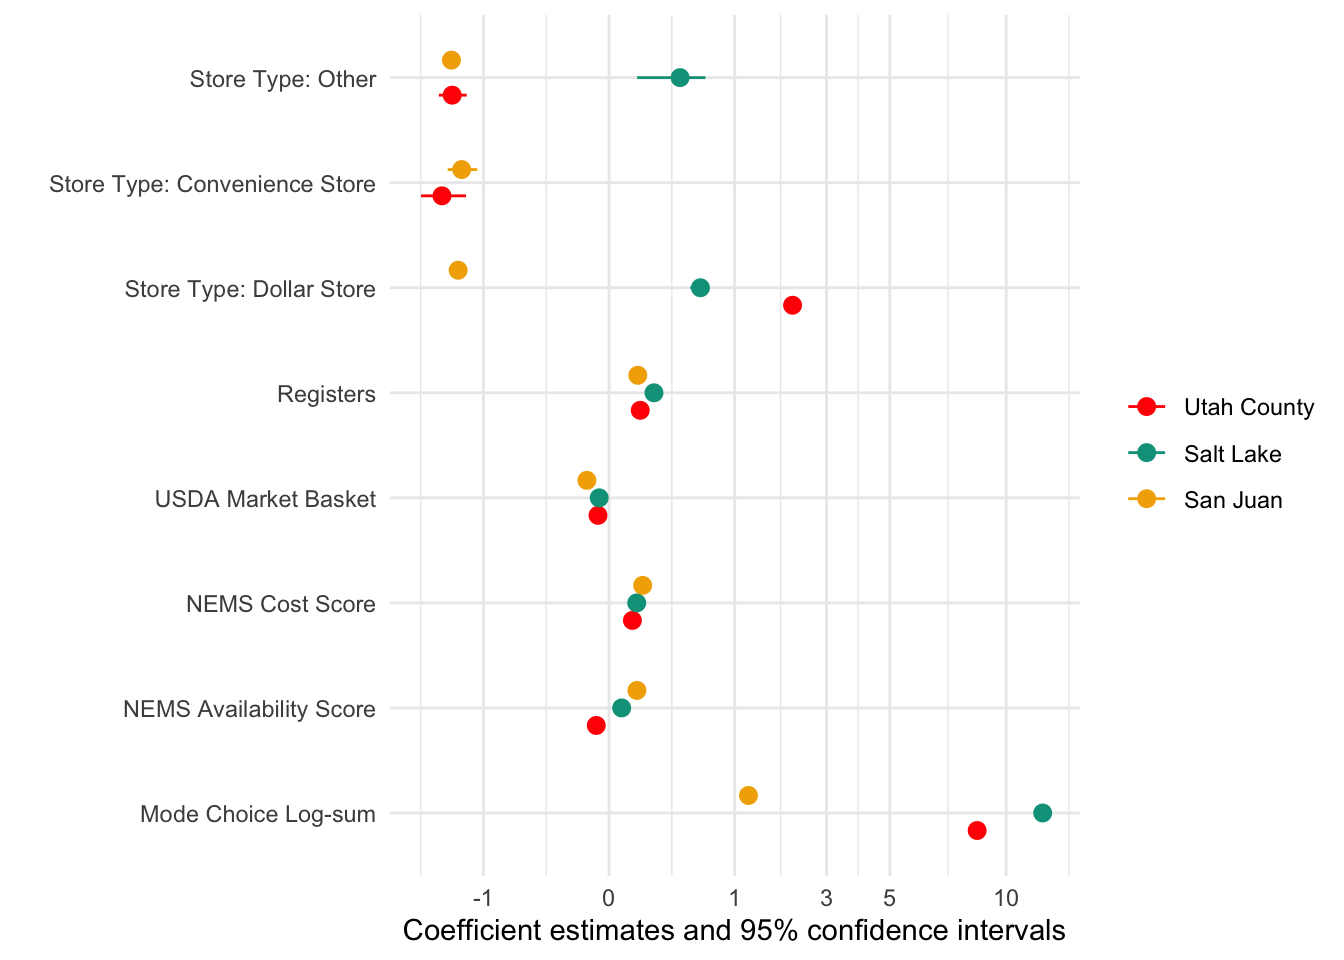
\includegraphics[width=6in,height=\textheight]{04_estimation_files/figure-pdf/fig-all-comp-1.pdf}

}

\caption{\label{fig-all-comp}Comparison of county model coefficient
estimates. Absolute square root transformation applied to improve
visibility.}

\end{figure}

To better visualize how the preferences in the three communities differ
from each other, Figure~\ref{fig-all-comp} plots the coefficient
estimates from the All model in each community. The mode choice log-sum
is strongly significant in all three communities, but it has its
smallest value in San Juan County where people often must travel long
distances to reach any stores. The highest mode choice log-sum value is
in Salt Lake, but this explains a smaller proportion of the model
outcomes than the lower value in Utah County; a possible hypothesis for
this observation may include the higher density of stores in Salt Lake
--- attributes are more important when so many stores are close together
--- paired with the somewhat lower vehicle ownership in that community
driving up the coefficient value. Most other estimates are somewhat
consistent across counties, with the exception of the NEMS variables
discussed previously and the role of dollar stores and other stores in
each community.

\hypertarget{sec-access}{%
\section{Accessibility}\label{sec-access}}

With the models estimated in Section~\ref{sec-estimation}, we can
evaluate the spatial access of each community. Figure~\ref{fig-map-ut}
shows the value of the grocery store destination choice log-sum for
block groups in Utah County. Unsurprisingly, the block groups in the
core of the urban areas of the region have the highest access to grocery
stores, because this is where the stores are located and also where the
transportation access to multiple destinations is highest. This map also
contains somewhat interesting implications for the equity of access. A
perhaps unique feature of Utah County's demographic geography is that
the wealthiest neighborhoods tend to be located on the mountain benches
east of the main urban areas. This means that in Utah County, at least,
the neighborhoods with the lowest access to grocery stores are actually
some of the wealthiest neighborhoods with the lowest concentrations of
ethnic minorities in the region.

\begin{figure}[t]

{\centering 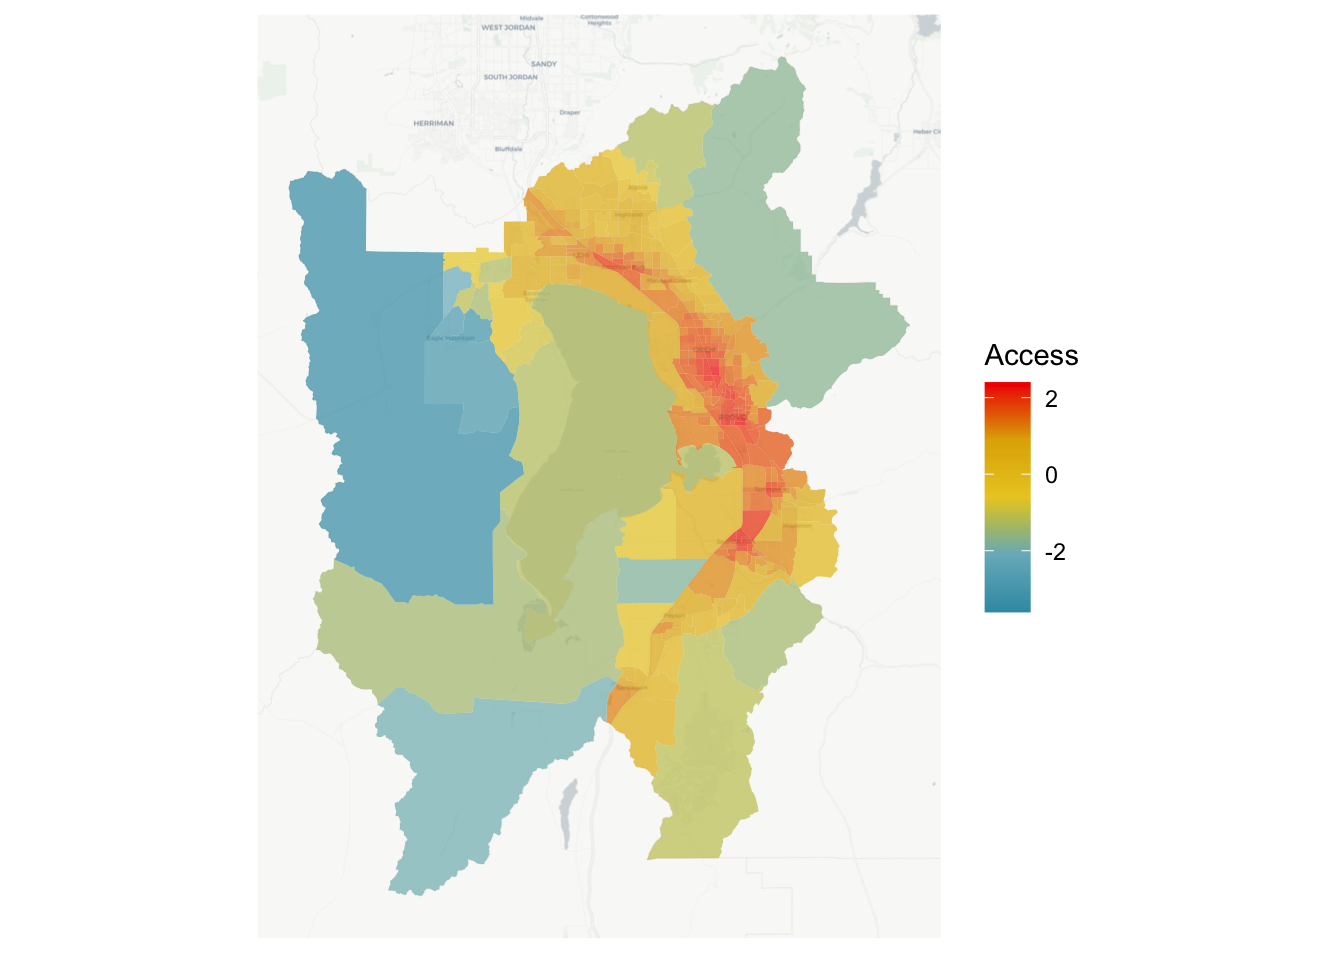
\includegraphics[width=6in,height=\textheight]{04_estimation_files/figure-pdf/fig-map-ut-1.pdf}

}

\caption{\label{fig-map-ut}Modeled access to grocery stores in Utah
County}

\end{figure}

Of course, much of this high access in the urban core of Utah County is
achieved by cheap and available automobile transportation. We can
consider what access looks like for those without cars by re-computing
the mode choice log-sum described in Section~\ref{sec-mcls} between all
block group / store pairs but eliding the automobile mode, and examining
the resulting impact to destination choice utility.
Figure~\ref{fig-map-nocar} shows the results of this analysis: whereas
the total access (with car included) is a smooth gradient across the
valley, the access for individuals without vehicles is blocky and
discontinuous, with neighborhoods of relatively good access immediately
next to neighborhoods with bad or non-existent access. This may reflect
the discontinuous nature of active transport and public transit
facilities in the region, as well as the auto-dominated locations of
many grocery stores. Note also that even for neighborhoods of relatively
good non-vehicle access, the destination choice log-sum value is
substantially lower than the logsum with vehicle access; the minimum
value on with vehicles is just below 0, whereas the \emph{maximum}
log-sum without vehicles is around -100. Because the log-sum occurs on
the same scale in both cases, this represents a serious additional cost
for non-vehicle users.

\begin{sidewaysfigure}

\begin{minipage}[t]{0.50\linewidth}

{\centering 

\raisebox{-\height}{

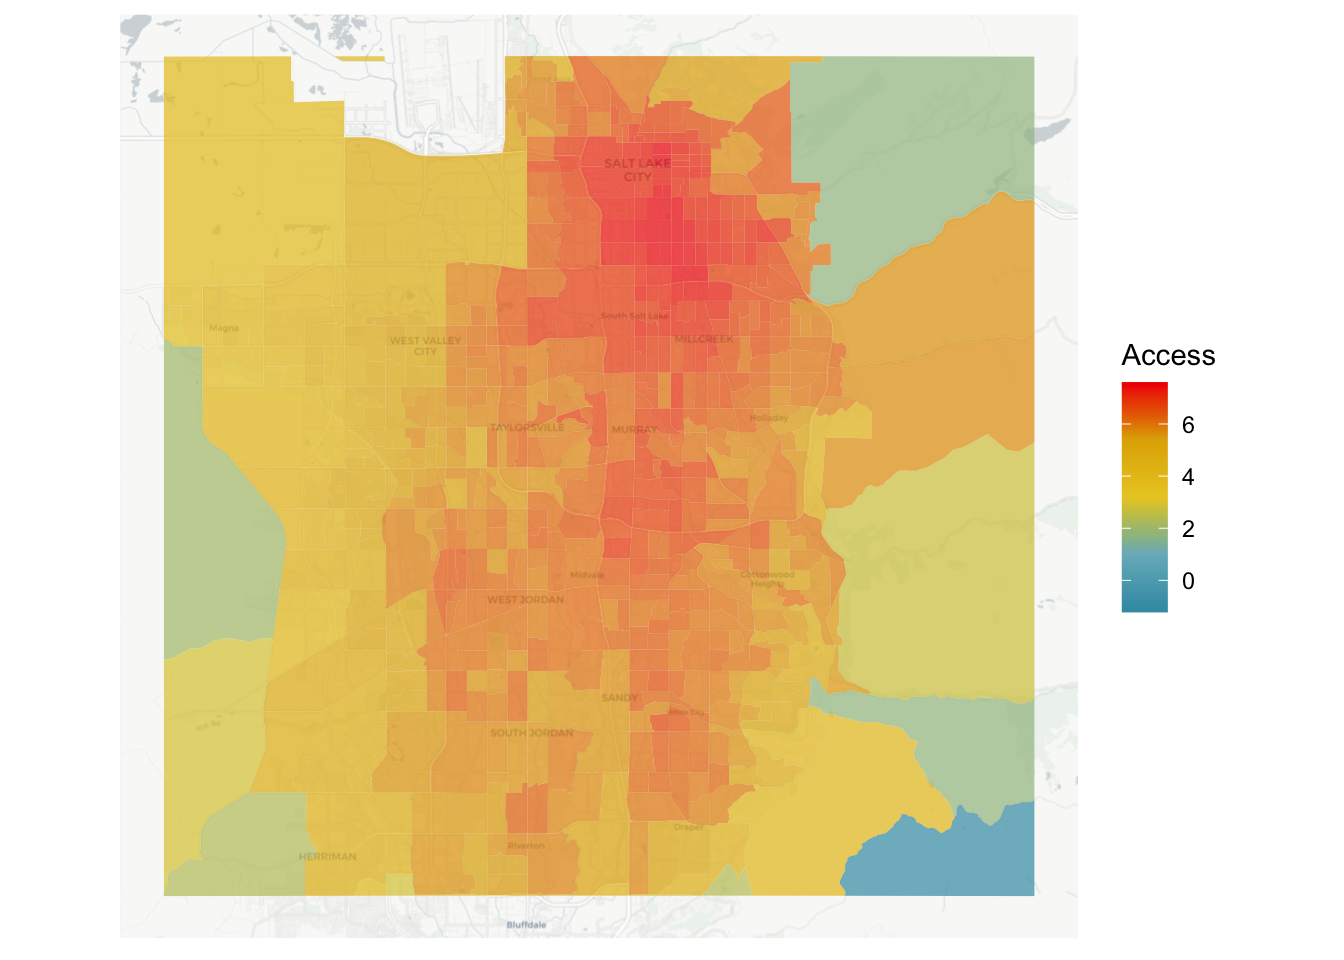
\includegraphics[width=4in,height=\textheight]{04_estimation_files/figure-pdf/fig-map-nocar-1.pdf}

}

}

\subcaption{\label{fig-map-nocar-1}With vehicles}
\end{minipage}%
%
\begin{minipage}[t]{0.50\linewidth}

{\centering 

\raisebox{-\height}{

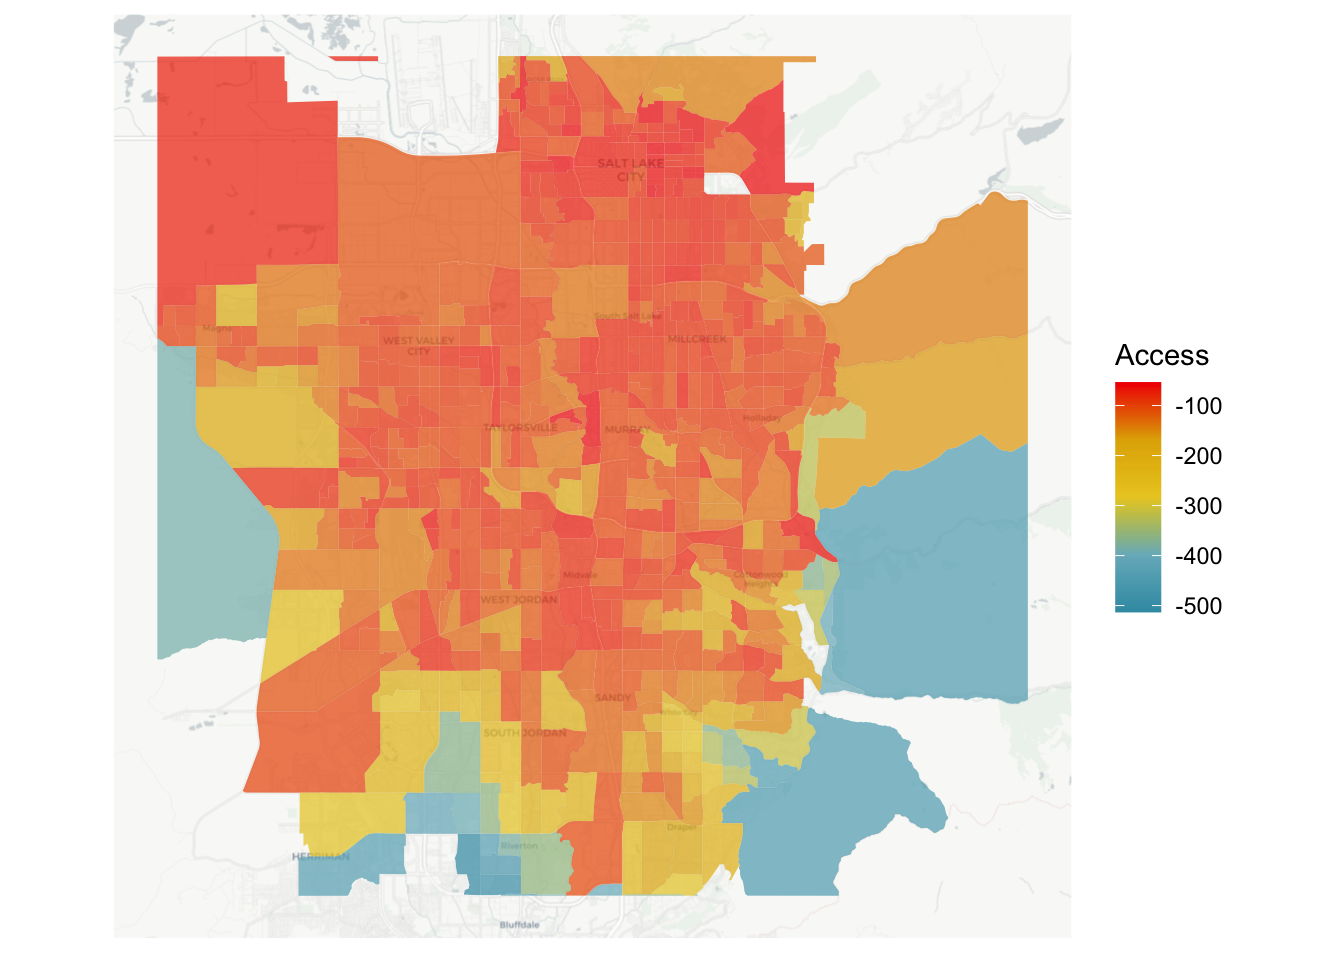
\includegraphics[width=4in,height=\textheight]{04_estimation_files/figure-pdf/fig-map-nocar-2.pdf}

}

}

\subcaption{\label{fig-map-nocar-2}Without vehicles}
\end{minipage}%

\caption{\label{fig-map-nocar}Access to groceries in Salt Lake County
with and without a vehicle.}

\end{sidewaysfigure}

\bookmarksetup{startatroot}

\hypertarget{sec-scenarios}{%
\chapter{Application}\label{sec-scenarios}}

In this section, we develop a series of scenarios to which we apply the
models estimated in Chapter~\ref{sec-results}. These scenarios are
constructed to ascertain what may be the best strategy to improve
nutrition access in a community. We first describe how each scenario was
constructed, and then discuss the results together.

The accessibility of each scenario was to be determined using the
approximated utility coefficients of the All model estimated in
Chapter~\ref{sec-results},
\begin{equation}\protect\hypertarget{eq-scenu}{}{
U_{ij}= \beta_{MCLS}( k_{ij}) +  \beta_{n-a} (\mathrm{NEMS-Availability}) +
  \beta_{n-c}\mathrm({NEMS-Cost}) + \\ \beta_{mkt} (\mathrm{Market Basket}) + \pmb{\beta}_{type}(\mathrm{Type})  
}\label{eq-scenu}\end{equation} and the total access benefit is defined
as the consumer surplus given in Equation~\ref{eq-cs}. Note that this
benefit is denominated in units of utility (Ben-Akiva and Lerman, 1985),
and the coefficients in Equation~\ref{eq-scenu} serve to convert between
the units of the variable and utility. Specifically, the \(\beta_{mkt}\)
coefficient represents how many dollars of grocery cost a person is
willing to spend to increase their utility by one unit.

In actuality, the utility formula in Equation~\ref{eq-scenu} is a
relative utility added by an unknown constant,
\(U_{ij} = f(\mathbf{\beta}, X_{ij}) + C\), but this \(C\) term is
included in all the alternatives and therefore cancels out (Train, 2009)
in estimation. This means we cannot asses the \emph{absolute} value of
utility, but we can assess the \emph{relative} monetary benefit of the
difference between two scenarios as \[
\mathrm{Benefit} = \sum_{i}\left(-\frac{\omega_i}{\beta_{mkt}}(CS_i^1 - CS_i^1)\right)
\] where a weight \(\omega\) accounts for the population in each origin
zone \(i\) and the \(\beta_{mkt}\) converts the difference in utility
into a dollar amount.

\hypertarget{scenario-descriptions}{%
\section{Scenario Descriptions}\label{scenario-descriptions}}

There are three general strategies we develop scenarios around:

\begin{enumerate}
\def\labelenumi{\arabic{enumi}.}
\tightlist
\item
  Erect a new grocery store in the community, in a place where one does
  not already exist.
\item
  Improve an existing convenience store or dollar store so that it has
  the attributes of a full-service grocery store.
\item
  Improve the transit and non-motorized access to stores in a region.
\end{enumerate}

We implement all three strategies in scenarios on the west Salt Lake
valley community. We also implement strategy 1 (a new store) in the San
Juan and Utah County communities for comparison.

\hypertarget{erect-a-new-store}{%
\subsection{Erect a new store}\label{erect-a-new-store}}

This strategy assumes that the nutrition environment would benefit from
a new store located in a place that presently has low grocery store
access. To examine the potential for this strategy to improve access to
nutrition in each community, we calculate the change in destination
choice log-sum when a new store is added to the region in a location
where access is currently poor. The new store is a full-service grocery
store with a number of registers equal to the mean of other grocery
stores in the community, and NEMS availability score, NEMS cost score,
and market basket cost equivalent to the 75\(^{th}\) percentile for the
community. Thus the store is expected to be better-than-average quality
as perceived by the residents of the community. The location for this
new store is at 4100 S and 2700 W in West Valley City.

\hypertarget{improve-an-existing-store}{%
\subsection{Improve an existing store}\label{improve-an-existing-store}}

This strategy assumes that existing stores are in locations that the
community values and can access, but that those stores may not have high
availability of quality goods. To examine the potential for this
strategy to improve access to nutrition, we improve the attributes of an
existing dollar store in the community so that it has the size, prices,
and availability of goods as a full-service grocery store. As above, we
create a full-service grocery store with a number of registers equal to
the mean of other grocery stores in the community, and NEMS availability
score, NEMS cost score, and market basket cost equivalent to the
75\(^{th}\) percentile for the community. Thus the store is expected to
be better-than-average quality as perceived by the residents of the
community; the difference from the previous scenario is that the
improved store takes the place of an existing convenience store or
dollar store.

The improved stores are at the following locations in each community:

\begin{itemize}
\tightlist
\item
  An ethnic store near 2700 W 3500 S in West Valley City (Salt Lake)
\item
  A small grocery store in Santaquin (Utah County)
\item
  A dollar store in Blanding (San Juan County)
\end{itemize}

\hypertarget{improve-transit-and-non-motorized-transport}{%
\subsection{Improve transit and non-motorized
transport}\label{improve-transit-and-non-motorized-transport}}

This strategy assumes that people cannot easily travel to existing
stores because they cannot or do not drive for a variety of reasons, and
that the public and and active transport networks provide an
insufficient level of service. To examine the potential for this
strategy to improve access to nutrition, we improve the travel time
costs in the Salt Lake community for non-motorized and public
transportation in the region and calculate the change in destination
choice log-sum.

For active transportation, the lack of pedestrian facilities across and
alongside roads both in reality and in the OpenStreetMap dataset may
substantially increase measured walk distances and times. In this
scenario, we replace the times measured from OpenStreetMap using R5 with
an idealized Euclidean distance function,
\begin{equation}\protect\hypertarget{eq-newwalk}{}{
t_{\mathrm{walk}} = \frac{\sqrt{2} * d'_{ij}}{v_{\mathrm{walk}}}
}\label{eq-newwalk}\end{equation} where \(d'_{ij}\) is the Euclidean
(straight-line) distance between \(i\) and \(j\) and \(v_{ij}\) is an
average walking speed equivalent to 3.5 feet per second (Fitzpatrick et
al., 2006). The distance is multiplied by the square root of 2 to
reflect the Manhattan distance (along a gridded street system). We
retain the cap on walking distance at 10 kilometers. Though this
distance may radically understate the real walking distance, we are
trying to create an idealized scenario of effectively frictionless
active transport. For public transit, we assume that the frequency of
service is such that all transfer and initial wait times are at most 5
minutes, and that no person must walk more than 10 minutes to access
their first public transport service.

Travel times are improved in this way for all block group --- store
pairs in the west Salt Lake Valley community.

\hypertarget{scenario-results}{%
\section{Scenario Results}\label{scenario-results}}

Using the methodology described above, we recalculated the destination
choice log-sum value for each block group under each scenario, and
compared the change in accessibility resulting from the improvement.

\begin{figure}[t]

{\centering 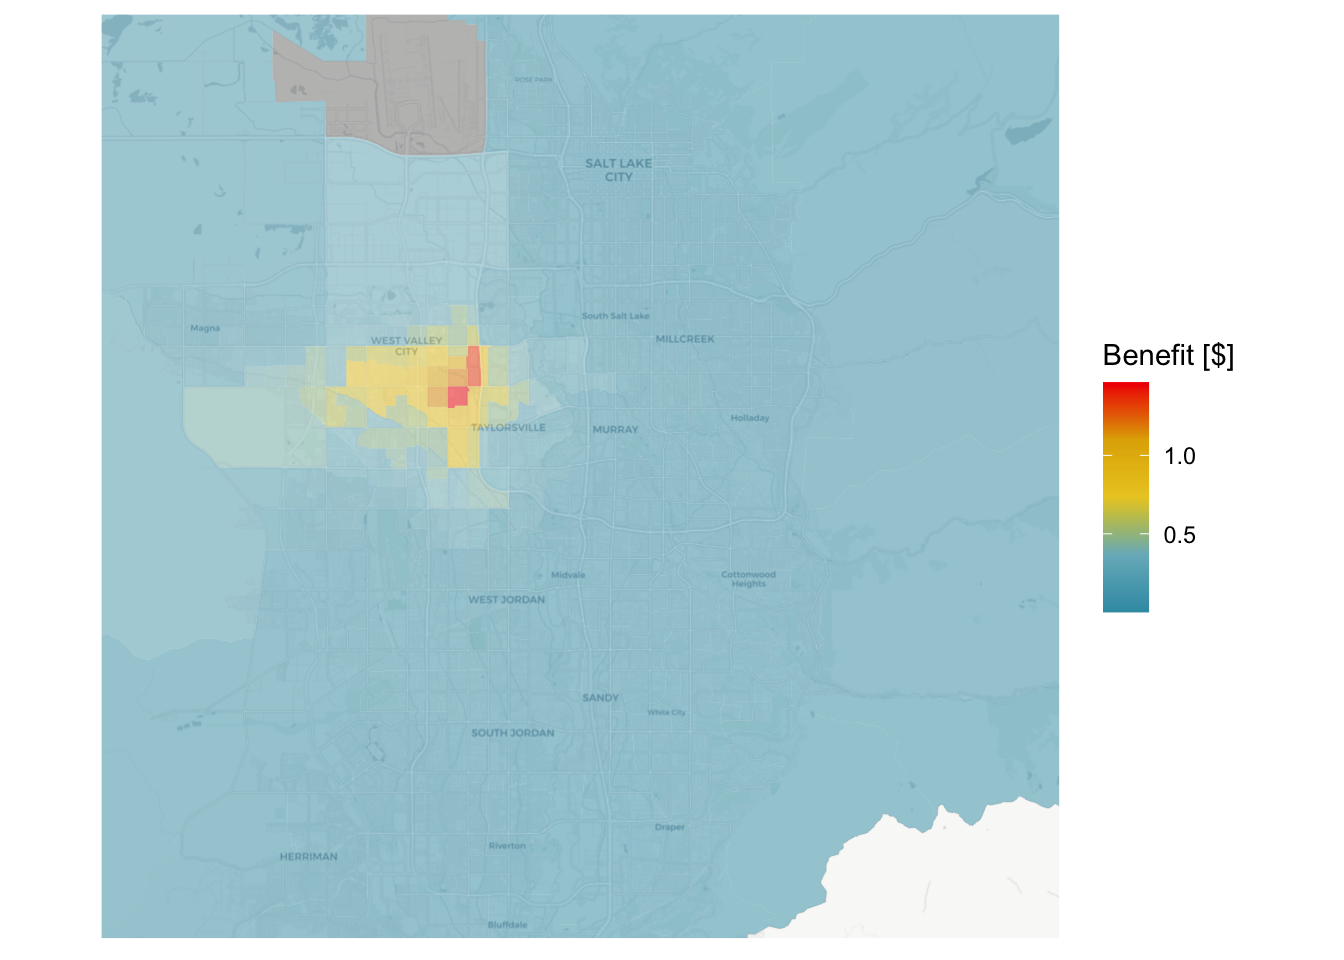
\includegraphics[width=6in,height=\textheight]{05_scenarios_files/figure-pdf/fig-s1results-1.pdf}

}

\caption{\label{fig-s1results}Estimated per-household benefits of adding
new full-service store in west Salt Lake Valley}

\end{figure}

Figure~\ref{fig-s1results} shows the geographic distribution of benefits
associated with locating a new store at a site in the Salt Lake
community. The benefits are largest immediately next to the new store,
where they exceed \(1\) for each household each time the household makes
a trip to a grocery store.

\begin{figure}[t]

{\centering 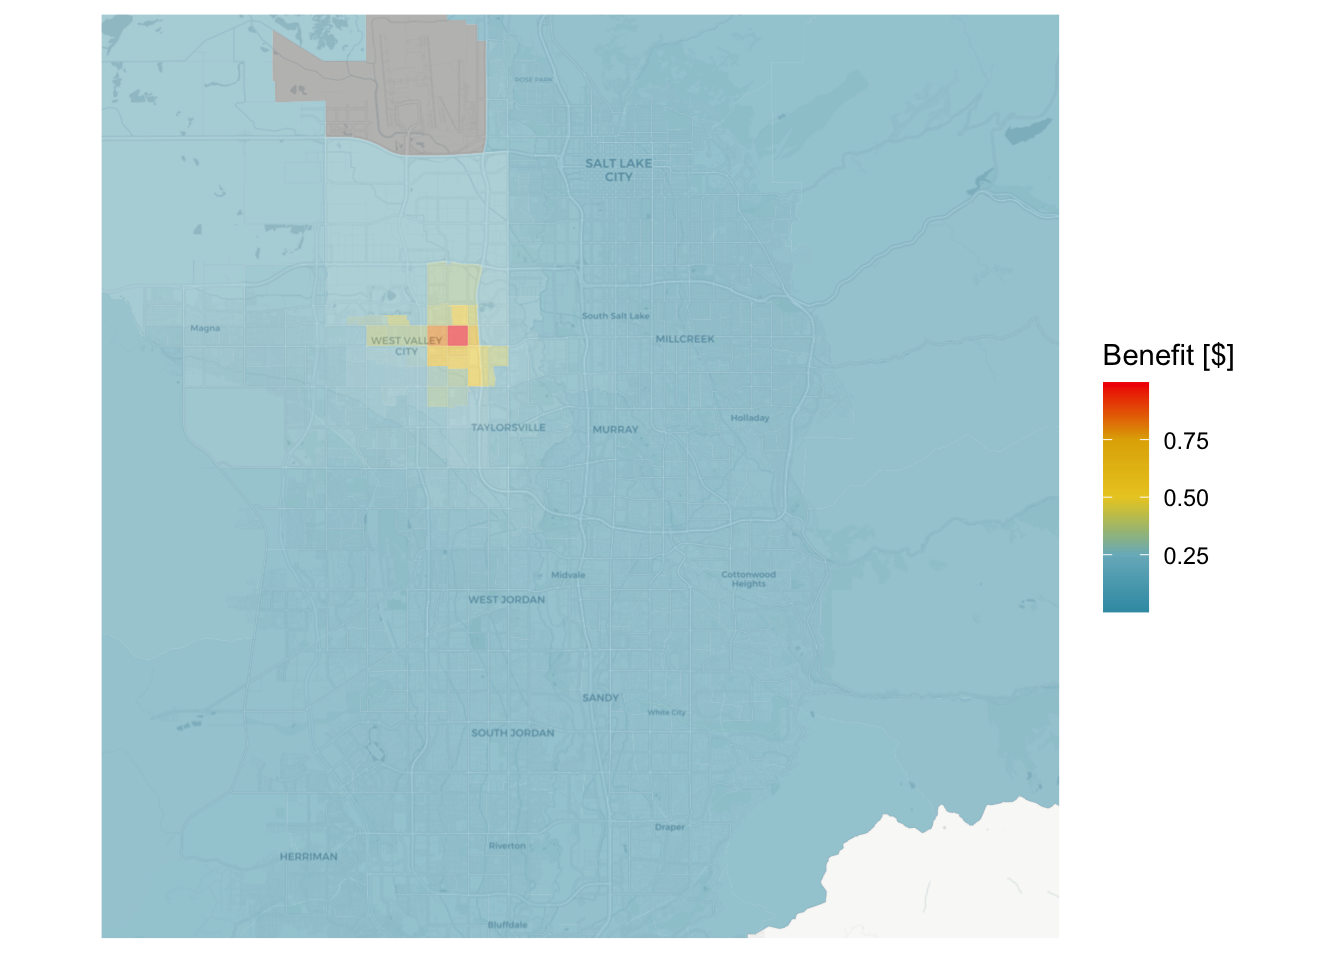
\includegraphics[width=6in,height=\textheight]{05_scenarios_files/figure-pdf/fig-s2results-1.pdf}

}

\caption{\label{fig-s2results}Estimated per-household benefits of
improving an existing store in west Salt Lake Valley}

\end{figure}

Figure~\ref{fig-s2results} shows the results of the scenario improving
an existing store in the Salt Lake community. Compared to the results of
the new store scenario, the scale of the benefits are not as substantial
(a maximum per-household-trip benefit of less than \$1), and seem to not
cover quite as large a geographic region. Figure~\ref{fig-s2sjut} shows
the results of improving a store in Utah and San Juan Counties. As in
Salt Lake, the benefits are most strongly concentrated in the immediate
vicinity of the improved store. One interesting observation ---
especially in Utah County --- is that the improvements are felt more
strongly in the block groups near the improved store that have lower
availability of other options. The block group in Utah County directly
containing the improvement sees a per-household-trip benefit well over
\$2, considerably more than the maximum benefit in Salt Lake. This is
intuitive, as the improvement of a store matters less if the stores
close to you are already sufficient.

\begin{sidewaysfigure}

\begin{minipage}[t]{0.50\linewidth}

{\centering 

\raisebox{-\height}{

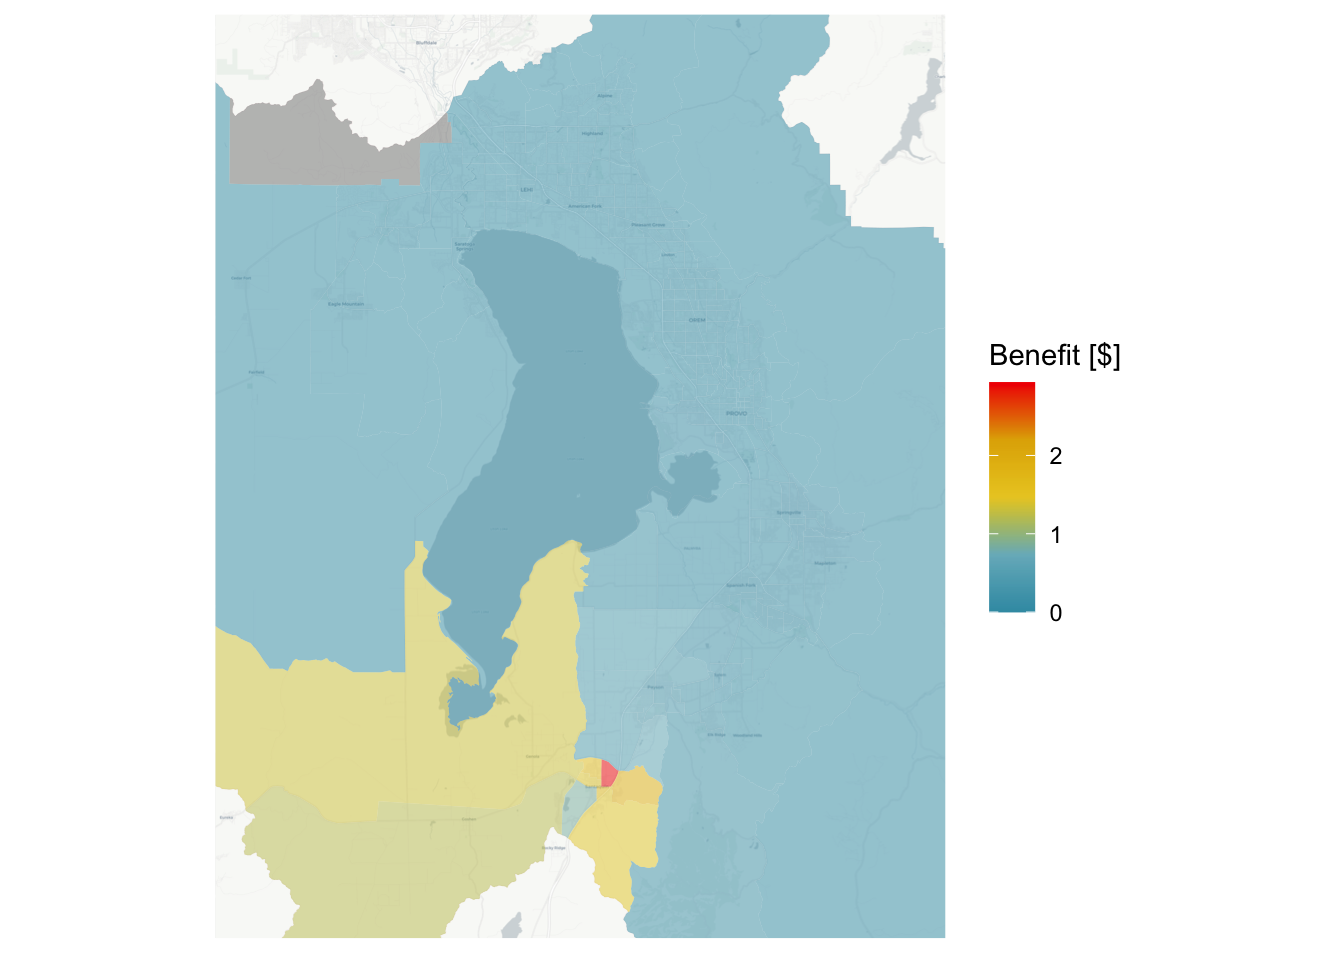
\includegraphics[width=4in,height=\textheight]{05_scenarios_files/figure-pdf/fig-s2sjut-1.pdf}

}

}

\subcaption{\label{fig-s2sjut-1}Utah County (in Santaquin)}
\end{minipage}%
%
\begin{minipage}[t]{0.50\linewidth}

{\centering 

\raisebox{-\height}{

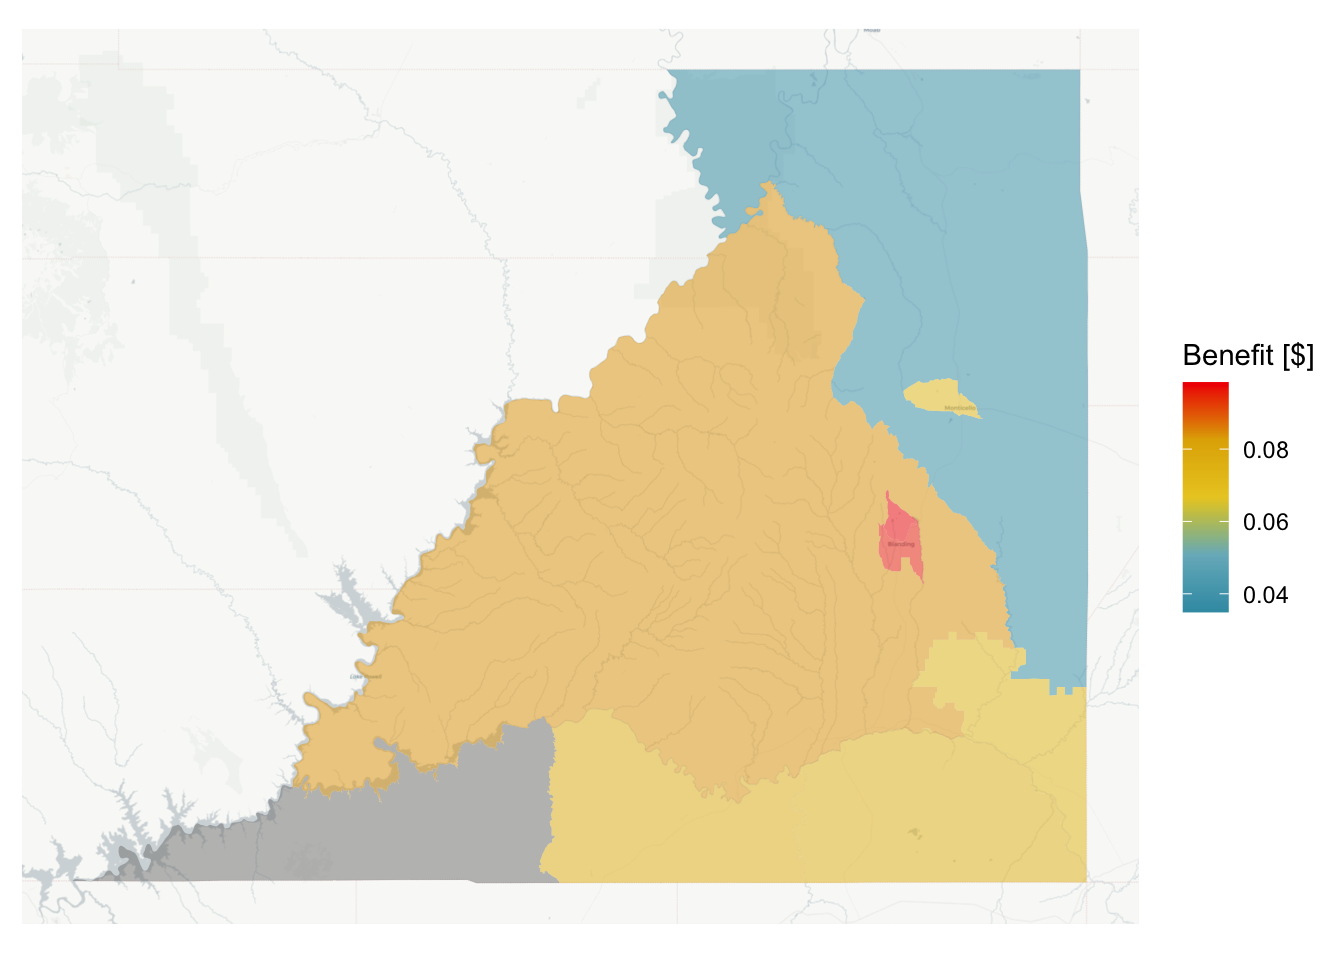
\includegraphics[width=4in,height=\textheight]{05_scenarios_files/figure-pdf/fig-s2sjut-2.pdf}

}

}

\subcaption{\label{fig-s2sjut-2}San Juan County (in Blanding)}
\end{minipage}%

\caption{\label{fig-s2sjut}Estimated per-household benefits of improving
an existing store in Utah and San Juan Counties.}

\end{sidewaysfigure}

The results of the third scenario, improving the access of non-motorized
and public transit access to stores, are shown in
Figure~\ref{fig-s3results}. This benefit is spread over a larger area,
and is concentrated on the 35 MAX bus rapid transit corridor where the
improvement in walk access time to transit couples with high frequency
transit service to large grocery stores on the corridor. The
per-household-trip benefit is very small however, with a maximum benefit
on the order of \$0.25.

\begin{figure}[t]

{\centering 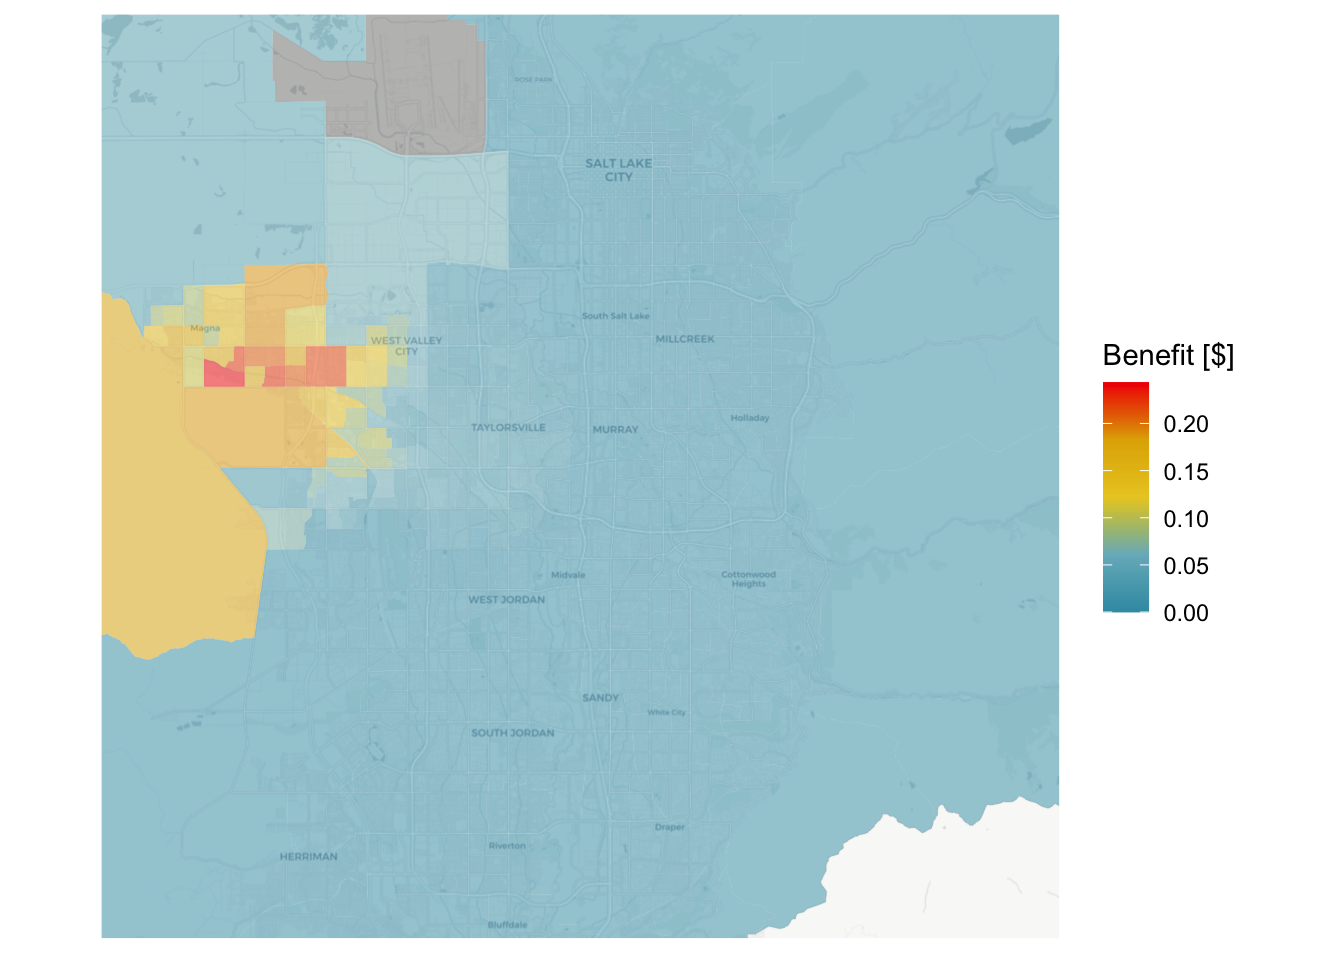
\includegraphics[width=6in,height=\textheight]{05_scenarios_files/figure-pdf/fig-s3results-1.pdf}

}

\caption{\label{fig-s3results}Estimated per-household benefits of
improving non-motorized and public transport access to groceries in Salt
Lake Valley.}

\end{figure}

\hypertarget{tbl-scenarios}{}
\begin{table}
\caption{\label{tbl-scenarios}Scenario Benefits }\tabularnewline

\centering
\begin{tabular}[t]{llll}
\toprule
\multicolumn{1}{c}{ } & \multicolumn{3}{c}{Weighted by} \\
\cmidrule(l{3pt}r{3pt}){2-4}
Scenario & Households & Non-white & Low-Income\\
\midrule
New Store & \$5,538,988 & \$2,449,404 & \$961,684\\
\addlinespace[0.3em]
\multicolumn{4}{l}{\textbf{Improved Store}}\\
\hspace{1em}Salt Lake Valley & \$2,849,176 & \$1,364,404 & \$569,364\\
\hspace{1em}Utah County & \$1,516,458 & \$245,638 & \$233,778\\
\hspace{1em}San Juan County & \$52,152.69 & \$26,914.35 & \$18,280.71\\
Improved Transport & \$872,015 & \$393,554 & \$120,078\\
\bottomrule
\end{tabular}
\end{table}

Although comparing the geographic distribution of benefits is helpful,
the aggregate benefit is more likely to guide policy. Additionally, the
aggregate benefits can be weighted in different ways to understand the
effects of the various policies on different populations.
Table~\ref{tbl-scenarios} presents the aggregate benefit from each of
the three scenarios (and the result of the second scenario in all three
communities). The Households column multiplies the difference in
destination choice log-sum at each block group by the number of
households in that block group, while the non-white and low-income
columns weight the difference by the share of non-white individuals and
low-income households respectively. All demographic data comes from the
American Community Survey 5-year aggregations.

These alternate weighting schemes help to illustrate the potential
equity of the benefit distribution should each scenario be pursued. The
new store scenario in the Salt Lake community, for example, has a total
benefit of approximately \$5.5 million. Of this amount, somewhat less
than half the benefits go to non-white individuals and less than
one-fifth to low-income households. These ratios are more or less the
same for the store improvement scenario and the improved transport
scenario in the Salt Lake Valley. The Utah County store improvement, on
the other hand, has a somewhat higher proportion of benefits going to
low-income households relative to non-white households. This is a
reflection of the lower minority population in southern Utah County vis
a vis west Salt Lake valley, but is nonetheless a metric that program
evaluators might pay attention to.

Overall, the improved store brings more than twice the benefits of
improving non-automobile transportation, and the new store more than
five times the benefits. Understanding the costs of these various
alternatives is outside the scope of this research, but the level of
infrastructure investment required to increase transportation level of
service to that constructed in the simulation is likely an order of
magnitude higher than the cost of a single new grocery store. It should
also be acknowledged that improving non-automobile infrastructure and
services would have benefits beyond just grocery store trips that we do
not attempt to enumerate here. It is also not clear whether the level of
improvement simulated in the second scenario could be accomplished
within the envelope of the existing store; it may be that such
improvements would meet or exceed the cost of building a new store on a
new site, along with stocking, staffing, and operating the store.

\bookmarksetup{startatroot}

\hypertarget{sec-conclude}{%
\chapter{Conclusions and Recommendations}\label{sec-conclude}}

As outlined in Chapter~\ref{sec-literature}, transportation agencies
seeking to improve the health and quality of life for residents must
consider not simply their mobility needs, but the safety of the
transportation system, the effects of the system on disadvantaged
populations, and the ability of residents to access quality community
resources. Access to nutrition is a critical topic that has been a
frequent focus of academic literature in public health, community
planning, and engineering, but the varying and incomplete quantitative
definitions of access have perhaps limited efforts at developing
solutions.

In this research, we explored an emerging technique to measure access to
nutrition in multiple communities in Utah that combines transport access
with the quality of markets, weighted against each other. We then used
this model to examine an array of targeted policies that would
potentially improve access to nutrition to a specific community.

This concluding section presents both a series of limitations to this
research with associated opportunities for future efforts, followed by
specific recommendations to the Utah Department of Transportation as it
seeks to pursue its mission to ``Enhance the Quality of Life through
Transportation.''

\hypertarget{sec-limitations}{%
\section{Limitations}\label{sec-limitations}}

A number of assumptions made in Chapter~\ref{sec-methods} lead to
limitations that other reasonable researchers might pursue differently,
and thereby obtain marginally different outcomes.

In selecting a survey instrument with which to collect the store
attribute data, we selected an existing and validated instrument from
the nutrition environment literature. The NEMS-S focus on low-calorie
and low-fat alternatives may be somewhat outdated in view of modern
nutritional guidelines. For example, the NEMS-S does not track the
availability and price of poultry, as ``lean'' poultry is not a goods
category in the way that ground beef comes with multiple fat contents.
Thus a major source of protein in typical American diets (FNS, 2021) was
not traced across stores in each community. On a more basic level, the
NEMS-S attempts to measure a store's stocking of goods that researchers
believe are beneficial, and does not measure either what people wish to
buy, or what they are actually buying at a store. Future research might
attempt to survey shoppers on what they actually purchased at each store
--- or collect receipts of their purchases --- though this would
substantially raise the difficulty of collecting data.

Most households do not obtain all their groceries at a single store,
though this research of necessity assumed that a simulated person chose
exactly one store from stores available to them. Similarly, the
location-based services data provided by StreetLight and used to
identify which stores people traveled to only reveal whether a device
was identified inside a geographic polygon, and not what they were
actually doing in that polygon. This research had no way of
distinguishing, for example, whether an individual device observed at a
dollar store or a super market (e.g.~Wal-Mart) was there to purchase
groceries or some other household goods that might not be offered at
more traditional food markets.

A number of simplifying assumptions concern the socioeconomic and
spatio-temporal detail supplied to the choice models and accessibility
calculators. The StreetLight data do not contain any demographic
information on the individuals making trips, beyond the inferences made
possible by the residence block group. This makes it difficult to
estimate whether lower income households are more or less sensitive to
travel distances or prices. Additionally, the research assumed that
every trip was from the population-weighted block group centroid, which
may vary substantially from the actual distance traveled, especially in
large block groups. The methodology also used travel times calculated in
the AM peak hour; though this time maximizes the availability of transit
options, it is not a typical peak time for grocery shopping. All of
these limitations could potentially be relaxed by using a synthetic
population with detailed socioeconomic data and parcel-level locations
determined by an activity-based model, as proposed by (Dong et al.,
2006). In this exercise, which we leave to future research, the grocery
maintenance trips could be explicitly modeled, with synthetic
individuals of unique characteristics choosing destinations that are
available on the course of their other daily activities, using their
chosen travel modes.

Finally, the scenarios presented in Chapter~\ref{sec-scenarios} are
designed to illustrate potential applications of this accessibility
methodology, with a comparative analysis of strategies to improve access
to nutrition. Selecting different sites, attribute levels, or transport
policies might substantially change the scale or rank-ordering of the
estimated benefits. A comprehensive search for the location that would
maximize benefits would be an interesting exercise, which we also leave
to future research.

\hypertarget{sec-recommend}{%
\section{Recommendations}\label{sec-recommend}}

This research results in two recommendations to the Utah Department of
Transportation and its partner agencies.

First, the research has underlined that communities in Utah have large
differences in their ability to access quality nutrition, and that many
communities --- especially in rural Utah --- travel long distances to
obtain quality goods. At some level, this is evidence that UDOT has
succeeded in its mobility-focused goals of connecting communities with
fluid and reliable transportation infrastructure. On a less encouraging
note, this observation also underscores the disparity in access defined
by the availability of automobiles with which to use this
infrastructure. For Utah households with limited vehicle availability,
access to nutrition is considerably constricted. The research also
revealed, however, that simply improving transit access and active
transportation paths might not be as beneficial as either improving the
quality of goods available in existing stores, or encouraging new store
locations. The role of UDOT in pursuing such policies needs to be
investigated. One potential strategy might be to alter access
management, highway prioritization, and other policies in a way that
encourages more stores with high-quality offerings in more communities.
This would alter the present pattern of locating large-scale stores near
arterial roadways, which maximizes the area over which a single store
can attract customers at the expense of neighborhood-level access.

At a methodological level, understanding the reasons why people
participate in activities, and their priorities in doing so, is a
necessary prerequisite to developing policies that improve the quality
of life. This is a transition from goals that simply seek to minimize
travel delay. To better facilitate and equip staff and researchers
considering these kinds of questions, UDOT should encourage and develop
activity-based approaches to travel forecasting. These approaches will
enable the more realistic analysis described in
Section~\ref{sec-limitations}, and provide better information for a host
of policies aimed at improving Utah's communities and their quality of
life.

\bookmarksetup{startatroot}

\hypertarget{acknowledgments}{%
\chapter*{Acknowledgments}\label{acknowledgments}}
\addcontentsline{toc}{chapter}{Acknowledgments}

\markboth{Acknowledgments}{Acknowledgments}

The authors acknowledge the Utah Department of Transportation (UDOT) for
funding this research, and the following individuals from UDOT and
partner agencies on the Technical Advisory Committee for helping to
guide the research: Kevin Nichol, Angelo Papastamos, Laura Holtrop-Kohl,
Brad Loveless, Chris Hall, Jay Aguilar, Jordan Backmon, Heidi LeBlanc,
Lea Palmer, and Ted Knowlton. The authors alone are responsible for the
preparation and accuracy of the information, data, analysis,
discussions, recommendations, and conclusions presented herein. The
contents do not necessarily reflect the views, opinions, endorsements,
or policies of the Utah Department of Transportation or the U.S.
Department of Transportation. The Utah Department of Transportation
makes no representation or warranty of any kind, and assumes no
liability therefore. Student research assistants who collected the store
data include Kaeli Monahan, Brooke Jones, and \ldots. Graphics in the
document are produced with multiple R packages (Arel-Bundock, 2022;
Dunnington, 2023; Ram and Wickham, 2018; Wickham, 2016).

\bookmarksetup{startatroot}

\hypertarget{references}{%
\chapter*{References}\label{references}}
\addcontentsline{toc}{chapter}{References}

\markboth{References}{References}

\hypertarget{refs}{}
\begin{CSLReferences}{1}{0}
\leavevmode\vadjust pre{\hypertarget{ref-aarts2006}{}}%
Aarts, L., van Schagen, I., 2006. Driving speed and the risk of road
crashes: {A} review. \emph{Accident Analysis \& Prevention} 38,
215--224. \url{https://doi.org/10.1016/j.aap.2005.07.004}

\leavevmode\vadjust pre{\hypertarget{ref-aggarwal2014}{}}%
Aggarwal, A., Cook, A.J., Jiao, J., Seguin, R.A., Vernez Moudon, A.,
Hurvitz, P.M., Drewnowski, A., 2014. Access to {Supermarkets} and
{Fruit} and {Vegetable Consumption}. \emph{American Journal of Public
Health} 104, 917--923. \url{https://doi.org/10.2105/AJPH.2013.301763}

\leavevmode\vadjust pre{\hypertarget{ref-algert2006}{}}%
Algert, S.J., Agrawal, A., Lewis, D.S., 2006. Disparities in {Access} to
{Fresh Produce} in {Low-Income Neighborhoods} in {Los Angeles}.
\emph{American Journal of Preventive Medicine} 30, 365--370.
\url{https://doi.org/10.1016/j.amepre.2006.01.009}

\leavevmode\vadjust pre{\hypertarget{ref-modelsummary}{}}%
Arel-Bundock, V., 2022. {modelsummary}: Data and model summaries in {R}.
\emph{Journal of Statistical Software} 103, 1--23.
\url{https://doi.org/10.18637/jss.v103.i01}

\leavevmode\vadjust pre{\hypertarget{ref-bao2020}{}}%
Bao, K.Y., Tong, D., Plane, D.A., Buechler, S., 2020. Urban food
accessibility and diversity: {Exploring} the role of small non-chain
grocers. \emph{Applied Geography} 125, 102275.
\url{https://doi.org/10.1016/j.apgeog.2020.102275}

\leavevmode\vadjust pre{\hypertarget{ref-barnes2021}{}}%
Barnes, M., 2021. Resiliency of {Utah}'s {Road Network}: {A Logit-Based
Approach} (\{\{MS Thesis\}\}). Brigham Young University, {Provo, Utah}.

\leavevmode\vadjust pre{\hypertarget{ref-ben-akiva1985}{}}%
Ben-Akiva, M., Lerman, S.R., 1985.
\href{https://www.jstor.org/stable/1391567}{Discrete {Choice Analysis}:
{Theory} and {Applications} to {Travel Demand}}. {MIT Press}.

\leavevmode\vadjust pre{\hypertarget{ref-bureauoflaborstatistics2023}{}}%
Bureau of Labor Statistics, 2023. 12-month percentage change, {Consumer
Price Index}, selected categories. \emph{Consumer Price Index}.

\leavevmode\vadjust pre{\hypertarget{ref-cass2005}{}}%
Cass, N., Shove, E., Urry, J., 2005. Social {Exclusion}, {Mobility} and
{Access}. \emph{The Sociological Review} 53, 539--555.
\url{https://doi.org/10.1111/j.1467-954X.2005.00565.x}

\leavevmode\vadjust pre{\hypertarget{ref-chakraborty2022}{}}%
Chakraborty, J., 2022. Children's exposure to vehicular pollution:
{Environmental} injustice in {Texas}, {USA}. \emph{Environmental
Research} 204, 112008.
\url{https://doi.org/10.1016/j.envres.2021.112008}

\leavevmode\vadjust pre{\hypertarget{ref-charreire2021}{}}%
Charreire, H., Roda, C., Feuillet, T., Piombini, A., Bardos, H., Rutter,
H., Compernolle, S., Mackenbach, J.D., Lakerveld, J., Oppert, J.M.,
2021. Walking, cycling, and public transport for commuting and
non-commuting travels across 5 {European} urban regions: {Modal} choice
correlates and motivations. \emph{Journal of Transport Geography} 96,
103196. \url{https://doi.org/10.1016/j.jtrangeo.2021.103196}

\leavevmode\vadjust pre{\hypertarget{ref-choma2021}{}}%
Choma, E.F., Evans, J.S., Gómez-Ibáñez, J.A., Di, Q., Schwartz, J.D.,
Hammitt, J.K., Spengler, J.D., 2021. Health benefits of decreases in
on-road transportation emissions in the {United States} from 2008 to
2017. \emph{Proceedings of the National Academy of Sciences} 118,
e2107402118. \url{https://doi.org/10.1073/pnas.2107402118}

\leavevmode\vadjust pre{\hypertarget{ref-clifton2004}{}}%
Clifton, K.J., 2004. Mobility {Strategies} and {Food Shopping} for
{Low-Income Families}: {A Case Study}. \emph{Journal of Planning
Education and Research} 23, 402--413.
\url{https://doi.org/10.1177/0739456X04264919}

\leavevmode\vadjust pre{\hypertarget{ref-cobbold2022}{}}%
Cobbold, A., Standen, C., Shepherd, L., Greaves, S., Crane, M., 2022.
Multimodal trips, quality of life and wellbeing: {An} exploratory
analysis. \emph{Journal of Transport \& Health} 24, 101330.
\url{https://doi.org/10.1016/j.jth.2022.101330}

\leavevmode\vadjust pre{\hypertarget{ref-conway2018}{}}%
Conway, M.W., Byrd, A., Eggermond, M. van, 2018. Accounting for
uncertainty and variation in accessibility metrics for public transport
sketch planning. \emph{Journal of Transport and Land Use} 11.
\url{https://doi.org/10.5198/jtlu.2018.1074}

\leavevmode\vadjust pre{\hypertarget{ref-conway2017}{}}%
Conway, M.W., Byrd, A., van der Linden, M., 2017. Evidence-{Based
Transit} and {Land Use Sketch Planning Using Interactive Accessibility
Methods} on {Combined Schedule} and {Headway-Based Networks}.
\emph{Transportation Research Record} 2653, 45--53.
\url{https://doi.org/10.3141/2653-06}

\leavevmode\vadjust pre{\hypertarget{ref-conway2019}{}}%
Conway, M.W., Stewart, A.F., 2019. Getting {Charlie} off the {MTA}: A
multiobjective optimization method to account for cost constraints in
public transit accessibility metrics. \emph{International Journal of
Geographical Information Science} 33, 1759--1787.
\url{https://doi.org/10.1080/13658816.2019.1605075}

\leavevmode\vadjust pre{\hypertarget{ref-mlogit}{}}%
Croissant, Y., 2020. Estimation of random utility models in {R}: The
{mlogit} package. \emph{Journal of Statistical Software} 95, 1--41.
\url{https://doi.org/10.18637/jss.v095.i11}

\leavevmode\vadjust pre{\hypertarget{ref-currie2010}{}}%
Currie, G., Delbosc, A., 2010. Modelling the social and psychological
impacts of transport disadvantage. \emph{Transportation} 37, 953--966.
\url{https://doi.org/10.1007/s11116-010-9280-2}

\leavevmode\vadjust pre{\hypertarget{ref-dedele2021}{}}%
Dėdelė, A., Miškinytė, A., 2021. Promoting {Sustainable Mobility}: {A
Perspective} from {Car} and {Public Transport Users}.
\emph{International Journal of Environmental Research and Public Health}
18, 4715. \url{https://doi.org/10.3390/ijerph18094715}

\leavevmode\vadjust pre{\hypertarget{ref-dhurandhar2021}{}}%
Dhurandhar, N.V., Petersen, K.S., Webster, C., 2021. Key {Causes} and
{Contributors} of {Obesity}: {A Perspective}. \emph{Nursing Clinics of
North America}, Obesity 56, 449--464.
\url{https://doi.org/10.1016/j.cnur.2021.07.007}

\leavevmode\vadjust pre{\hypertarget{ref-dong2006}{}}%
Dong, X., Ben-Akiva, M.E., Bowman, J.L., Walker, J.L., 2006. Moving from
trip-based to activity-based measures of accessibility.
\emph{Transportation Research Part A: Policy and Practice} 40, 163--180.
\url{https://doi.org/10.1016/j.tra.2005.05.002}

\leavevmode\vadjust pre{\hypertarget{ref-dons2018}{}}%
Dons, E., Rojas-Rueda, D., Anaya-Boig, E., Avila-Palencia, I., Brand,
C., Cole-Hunter, T., de Nazelle, A., Eriksson, U., Gaupp-Berghausen, M.,
Gerike, R., Kahlmeier, S., Laeremans, M., Mueller, N., Nawrot, T.,
Nieuwenhuijsen, M.J., Orjuela, J.P., Racioppi, F., Raser, E., Standaert,
A., Int Panis, L., Götschi, T., 2018. Transport mode choice and body
mass index: {Cross-sectional} and longitudinal evidence from a
{European-wide} study. \emph{Environment International} 119, 109--116.
\url{https://doi.org/10.1016/j.envint.2018.06.023}

\leavevmode\vadjust pre{\hypertarget{ref-ggspatial}{}}%
Dunnington, D., 2023.
\href{https://CRAN.R-project.org/package=ggspatial}{Ggspatial: Spatial
data framework for ggplot2}.

\leavevmode\vadjust pre{\hypertarget{ref-environmentalprotectionagency2023}{}}%
Environmental Protection Agency, 2023. Nonattainment {Areas} for
{Criteria Pollutants} ({Green Book}).

\leavevmode\vadjust pre{\hypertarget{ref-ermagun2020}{}}%
Ermagun, A., Tilahun, N., 2020. Equity of transit accessibility across
{Chicago}. \emph{Transportation Research Part D: Transport and
Environment} 86, 102461. \url{https://doi.org/10.1016/j.trd.2020.102461}

\leavevmode\vadjust pre{\hypertarget{ref-fann2013}{}}%
Fann, N., Fulcher, C.M., Baker, K., 2013. The {Recent} and {Future
Health Burden} of {Air Pollution Apportioned Across U}.{S}. {Sectors}.
\emph{Environmental Science \& Technology} 47, 3580--3589.
\url{https://doi.org/10.1021/es304831q}

\leavevmode\vadjust pre{\hypertarget{ref-finkel2020}{}}%
Finkel, E., McCormick, C., Mitman, M., Abel, S., Clark, J., 2020.
Integrating the {Safe System Approach} with the {Highway Safety
Improvement Program}: {An Informational Report} (No. FHWA-SA-20-018).
{Federal Highway Administration}, {Washington, D.C}.

\leavevmode\vadjust pre{\hypertarget{ref-fitzpatrick2006}{}}%
Fitzpatrick, K., Brewer, M.A., Turner, S., 2006. Another {Look} at
{Pedestrian Walking Speed}. \emph{Transportation Research Record} 1982,
21--29. \url{https://doi.org/10.1177/0361198106198200104}

\leavevmode\vadjust pre{\hypertarget{ref-fns2021}{}}%
FNS, 2021. Thrifty {Food Plan}. {Food and Nutrition Service, United
States Department of Agriculture}.

\leavevmode\vadjust pre{\hypertarget{ref-francis2012}{}}%
Francis, J., Wood, L.J., Knuiman, M., Giles-Corti, B., 2012. Quality or
quantity? {Exploring} the relationship between {Public Open Space}
attributes and mental health in {Perth}, {Western Australia}.
\emph{Social Science \& Medicine} 74, 1570--1577.
\url{https://doi.org/10.1016/j.socscimed.2012.01.032}

\leavevmode\vadjust pre{\hypertarget{ref-gerike2019}{}}%
Gerike, R., de Nazelle, A., Wittwer, R., Parkin, J., 2019. Special
{Issue} {``{Walking} and {Cycling} for better {Transport}, {Health} and
the {Environment}.''} \emph{Transportation Research Part A: Policy and
Practice}, Walking and {Cycling} for better {Transport}, {Health} and
the {Environment} 123, 1--6.
\url{https://doi.org/10.1016/j.tra.2019.02.010}

\leavevmode\vadjust pre{\hypertarget{ref-geurs2010}{}}%
Geurs, K., Zondag, B., de Jong, G., de Bok, M., 2010. Accessibility
appraisal of land-use/transport policy strategies: {More} than just
adding up travel-time savings. \emph{Transportation Research Part D:
Transport and Environment} 15, 382--393.
\url{https://doi.org/10.1016/j.trd.2010.04.006}

\leavevmode\vadjust pre{\hypertarget{ref-glanz2007}{}}%
Glanz, K., Sallis, J.F., Saelens, B.E., Frank, L.D., 2007. Nutrition
{Environment Measures Survey} in {Stores} ({NEMS-S}): {Development} and
{Evaluation}. \emph{American Journal of Preventive Medicine} 32,
282--289. \url{https://doi.org/10.1016/j.amepre.2006.12.019}

\leavevmode\vadjust pre{\hypertarget{ref-grengs2015}{}}%
Grengs, J., 2015. Nonwork {Accessibility} as a {Social Equity
Indicator}. \emph{International Journal of Sustainable Transportation}
9, 1--14. \url{https://doi.org/10.1080/15568318.2012.719582}

\leavevmode\vadjust pre{\hypertarget{ref-handy1997}{}}%
Handy, S.L., Niemeier, D.A., 1997. Measuring accessibility: {An}
exploration of issues and alternatives. \emph{Environment and Planning
A: Economy and Space} 29, 1175--1194.
\url{https://doi.org/10.1068/a291175}

\leavevmode\vadjust pre{\hypertarget{ref-hedrick2022}{}}%
Hedrick, V.E., Farris, A.R., Houghtaling, B., Mann, G., Misyak, S.A.,
2022. Validity of a {Market Basket Assessment Tool} for {Use} in
{Supplemental Nutrition Assistance Program Education Healthy Retail
Initiatives}. \emph{Journal of Nutrition Education and Behavior} 54,
776--783. \url{https://doi.org/10.1016/j.jneb.2022.02.018}

\leavevmode\vadjust pre{\hypertarget{ref-hillier2011}{}}%
Hillier, A., Cannuscio, C.C., Karpyn, A., McLaughlin, J., Chilton, M.,
Glanz, K., 2011. How {Far Do Low-Income Parents Travel} to {Shop} for
{Food}? {Empirical Evidence} from {Two Urban Neighborhoods}. \emph{Urban
Geography} 32, 712--729.
\url{https://doi.org/10.2747/0272-3638.32.5.712}

\leavevmode\vadjust pre{\hypertarget{ref-hu2015}{}}%
Hu, L., 2015. Job {Accessibility} of the {Poor} in {Los Angeles}.
\emph{Journal of the American Planning Association} 81, 30--45.
\url{https://doi.org/10.1080/01944363.2015.1042014}

\leavevmode\vadjust pre{\hypertarget{ref-jarry2021}{}}%
Jarry, V., Apparicio, P., 2021. Ride in {Peace}: {How Cycling
Infrastructure Types Affect Traffic Conflict Occurrence} in {Montréal},
{Canada}. \emph{Safety} 7, 63.
\url{https://doi.org/10.3390/safety7030063}

\leavevmode\vadjust pre{\hypertarget{ref-kaczynski2016}{}}%
Kaczynski, A.T., Schipperijn, J., Hipp, J.A., Besenyi, G.M., Wilhelm
Stanis, S.A., Hughey, S.M., Wilcox, S., 2016. {ParkIndex}: {Development}
of a standardized metric of park access for research and planning.
\emph{Preventive Medicine} 87, 110--114.
\url{https://doi.org/10.1016/j.ypmed.2016.02.012}

\leavevmode\vadjust pre{\hypertarget{ref-liu2022}{}}%
Liu, B., Widener, M.J., Smith, L.G., Farber, S., Minaker, L.M.,
Patterson, Z., Larsen, K., Gilliland, J., 2022. Disentangling {Time
Use}, {Food Environment}, and {Food Behaviors Using Multi-Channel
Sequence Analysis}. \emph{Geographical Analysis} 54, 881--917.
\url{https://doi.org/10.1111/gean.12305}

\leavevmode\vadjust pre{\hypertarget{ref-logan2019}{}}%
Logan, T., Williams, T., Nisbet, A., Liberman, K., Zuo, C., Guikema, S.,
2019. Evaluating urban accessibility: Leveraging open-source data and
analytics to overcome existing limitations. \emph{Environment and
Planning B: Urban Analytics and City Science} 46, 897--913.
\url{https://doi.org/10.1177/2399808317736528}

\leavevmode\vadjust pre{\hypertarget{ref-losada-rojas2021}{}}%
Losada-Rojas, L.L., Ke, Y., Pyrialakou, V.D., Konstantina Gkritza, 2021.
Access to healthy food in urban and rural areas: {An} empirical
analysis. \emph{Journal of Transport \& Health} 23, 101245.
\url{https://doi.org/10.1016/j.jth.2021.101245}

\leavevmode\vadjust pre{\hypertarget{ref-lunsford2021}{}}%
Lunsford, J., Brunt, A., Foote, J., Rhee, Y., Strand, M., Segall, M.,
2021. Analysis of {Availability}, {Quality}, and {Price} of {Food
Options} in {Denver}, {CO Grocery Stores}. \emph{Journal of Hunger \&
Environmental Nutrition} 16, 297--303.
\url{https://doi.org/10.1080/19320248.2020.1741482}

\leavevmode\vadjust pre{\hypertarget{ref-macfarlane2022a}{}}%
Macfarlane, G., Voulgaris, C.T., Tapia, T., 2022. City parks and slow
streets: {A} utility-based access and equity analysis. \emph{Journal of
Transport and Land Use} 15, 587--612.
\url{https://doi.org/10.5198/jtlu.2022.2009}

\leavevmode\vadjust pre{\hypertarget{ref-madzia2019}{}}%
Madzia, J., Ryan, P., Yolton, K., Percy, Z., Newman, N., LeMasters, G.,
Brokamp, C., 2019. Residential {Greenspace Association} with {Childhood
Behavioral Outcomes}. \emph{The Journal of Pediatrics} 207, 233--240.
\url{https://doi.org/10.1016/j.jpeds.2018.10.061}

\leavevmode\vadjust pre{\hypertarget{ref-mcfadden1974}{}}%
McFadden, D., 1974. Conditional logit analysis of qualitative choice
behavior, in: Zarembka, P. (Ed.), Frontiers in {Econometrics}. {Academic
Press}, pp. 105--142.

\leavevmode\vadjust pre{\hypertarget{ref-monfort2021}{}}%
Monfort, S.S., Cicchino, J.B., Patton, D., 2021. Weekday bicycle traffic
and crash rates during the {COVID-19} pandemic. \emph{Journal of
Transport \& Health} 23, 101289.
\url{https://doi.org/10.1016/j.jth.2021.101289}

\leavevmode\vadjust pre{\hypertarget{ref-nationalhighwaytrafficsafetyadministration2022}{}}%
National Highway Traffic Safety Administration, 2022. Countermeasures
that {Work}: {Distracted Driving}.

\leavevmode\vadjust pre{\hypertarget{ref-pereira2021}{}}%
Pereira, R.H.M., Saraiva, M., Herszenhut, D., Braga, C.K.V., Conway,
M.W., 2021. R5r: {Rapid Realistic Routing} on {Multimodal Transport
Networks} with {R}{\textsuperscript{5}} in {R}. \emph{Findings}.
\url{https://doi.org/10.32866/001c.21262}

\leavevmode\vadjust pre{\hypertarget{ref-wesanderson}{}}%
Ram, K., Wickham, H., 2018.
\href{https://CRAN.R-project.org/package=wesanderson}{Wesanderson: A wes
anderson palette generator}.

\leavevmode\vadjust pre{\hypertarget{ref-recker1978}{}}%
Recker, W.W., Kostyniuk, L.P., 1978. Factors influencing destination
choice for the urban grocery shopping trip. \emph{Transportation} 7,
19--33. \url{https://doi.org/10.1007/BF00148369}

\leavevmode\vadjust pre{\hypertarget{ref-schraufnagel2019}{}}%
Schraufnagel, D.E., Balmes, J.R., Cowl, C.T., De Matteis, S., Jung,
S.-H., Mortimer, K., Perez-Padilla, R., Rice, M.B., Riojas-Rodriguez,
H., Sood, A., Thurston, G.D., To, T., Vanker, A., Wuebbles, D.J., 2019.
Air {Pollution} and {Noncommunicable Diseases}: {A Review} by the
{Forum} of {International Respiratory Societies}' {Environmental
Committee}, {Part} 1: {The Damaging Effects} of {Air Pollution}.
\emph{Chest} 155, 409--416.
\url{https://doi.org/10.1016/j.chest.2018.10.042}

\leavevmode\vadjust pre{\hypertarget{ref-schwanen2015}{}}%
Schwanen, T., Lucas, K., Akyelken, N., Cisternas Solsona, D., Carrasco,
J.-A., Neutens, T., 2015. Rethinking the links between social exclusion
and transport disadvantage through the lens of social capital.
\emph{Transportation Research Part A: Policy and Practice} 74, 123--135.
\url{https://doi.org/10.1016/j.tra.2015.02.012}

\leavevmode\vadjust pre{\hypertarget{ref-smartgrowthamerica2023}{}}%
Smart Growth America, 2023. Complete {Streets Policy Framework}.
\emph{Smart Growth America}.

\leavevmode\vadjust pre{\hypertarget{ref-train2009}{}}%
Train, K.E., 2009. Discrete {Choice Methods} with {Simulation}, 2nd
edition. ed. {Cambridge University Press}, {Cambridge ; New York}.

\leavevmode\vadjust pre{\hypertarget{ref-udot2023}{}}%
UDOT, 2023b. Zero {Fatalities}: {Up-to-date} fatality and serious injury
data. \emph{Zero Fatalities}.

\leavevmode\vadjust pre{\hypertarget{ref-udot2023a}{}}%
UDOT, 2023a. Utah {Department} of {Transportation}: {About Us}.
\emph{UDOT}.

\leavevmode\vadjust pre{\hypertarget{ref-usdepartmentoftransportation2022}{}}%
US Department of Transportation, 2022. Transportation and {Health Tool}.

\leavevmode\vadjust pre{\hypertarget{ref-mice}{}}%
van Buuren, S., Groothuis-Oudshoorn, K., 2011. {mice}: Multivariate
imputation by chained equations in r. \emph{Journal of Statistical
Software} 45, 1--67. \url{https://doi.org/10.18637/jss.v045.i03}

\leavevmode\vadjust pre{\hypertarget{ref-visionzeronetwork2022}{}}%
Vision Zero Network, 2022. Vision {Zero Network}. \emph{Vision Zero
Network}.

\leavevmode\vadjust pre{\hypertarget{ref-ggplot2}{}}%
Wickham, H., 2016. \href{https://ggplot2.tidyverse.org}{ggplot2: Elegant
graphics for data analysis}. Springer-Verlag New York.

\leavevmode\vadjust pre{\hypertarget{ref-witten2003}{}}%
Witten, K., Exeter, D., Field, A., 2003. The {Quality} of {Urban
Environments}: {Mapping Variation} in {Access} to {Community Resources}.
\emph{Urban Studies} 40, 161--177.
\url{https://doi.org/10.1080/00420980220080221}

\leavevmode\vadjust pre{\hypertarget{ref-zerofatalities2022}{}}%
Zero Fatalities, 2022. Zero {Fatalities}. \emph{Zero Fatalities}.

\end{CSLReferences}



\end{document}
